\PassOptionsToPackage{quiet}{xeCJK}
\documentclass[withoutpreface,bwprint]{cumcmthesis}
\setCJKmainfont{SimSun.ttf}[AutoFakeBold]
\usepackage{etoolbox}
\usepackage{float}
\BeforeBeginEnvironment{tabular}{\zihao{-5}}
\usepackage[numbers,sort&compress]{natbib}  % 文献管理宏包
\usepackage[framemethod=TikZ]{mdframed}  % 框架宏包
\usepackage{url}  % 网页链接宏包
\usepackage{subcaption}  % 子图宏包
\newcolumntype{C}{>{\centering\arraybackslash}X}
\newcolumntype{R}{>{\raggedleft\arraybackslash}X}
\newcolumntype{L}{>{\raggedright\arraybackslash}X}

\title{基于双光束干涉和多光束干涉模型的外延层厚度的高精度测算与对比研究}  % 论文标题
\tihao{B}  % 题号
\baominghao{202527001171}  % 报名号
\schoolname{西安交通大学}  % 学校
\membera{李冬阳}  % 队员a
\memberb{曹芷维}  % 队员b
\memberc{朱韵桐}  % 队员c
\supervisor{陈磊}  % 指导老师
\yearinput{2025}
\monthinput{9}
\dayinput{7}
\begin{document}


\maketitle

\begin{abstract}
本文围绕碳化硅外延层厚度的测量这一问题,以\textbf{红外干涉法}为主要手段,针对双光束干涉和多光束干涉的不同情景分别建立数学模型并设计厚度求解方案,旨在制定一套科学、准确、可靠的碳化硅外延层厚度测试标准。


\textbf{对于问题一,}基于光在外延层-衬底只发生一次反射的\textbf{双光束干涉}的情景,我们利用干涉的基本原理,由几何关系推得光程差,进而推导出双波束相位差,并利用\textbf{斯涅尔折射定律}和干涉条件下的相位差所满足的关系式,建立起红外光谱的波长、外延层的折射率和红外光的入射角等参数与外延层厚度相关联的数学模型,为厚度计算提供理论基础。

\textbf{对于问题二,}基于问题一所建立的数学模型,设计了外延层厚度的算法,并将附件1和附件2的数据可视化处理,利用\textbf{傅里叶变换}提取周期。同时结合\textbf{菲涅尔公式}精确计算折射率数据,算得外延层厚度为7.4837$\mu\text{m}$,通过模型的检验和计算过程的分析,验证模型的可靠性与准确性。

\textbf{对于问题三,}基于光学理论分析,推导出多光束干涉下反射率的特性及其发生的必要条件。多光束干涉情况下,反射率-波数图像表现出不对称性,但波谷分布位置与双光束干涉相同。利用此特性,对附件3和附件4中硅晶圆的反射率数据进行分析,准确计算硅外延层厚度为$\ 3.9270\ \mu\text{m}$。同时,提取多光束干涉的特征并设计相应数学模型及算法。计算结果表明,多光束干涉能\textbf{提升厚度计算的精度}。针对碳化硅晶圆片(附件1和附件2)数据分析,认为多光束干涉影响可忽略,\textbf{仅发生双光束干涉}。

该研究系统性地建立了双光束及多光束干涉模型,设计了相应的厚度求解方法,并通过实验数据验证,具有较高的科学性和应用价值。


\keywords{光的干涉\quad  菲涅尔定律\quad  高斯滤波\quad  傅里叶变换\quad  时间序列分析}
\end{abstract}

\section{问题重述}
\subsection{问题背景}
碳化硅(SiC)作为第三代半导体材料,因其优异的物理与电学性能,在高温、高压、高频等极端工况下展现出巨大潜力。外延层厚度是SiC器件设计与制造中的关键参数,直接影响器件的核心性能指标。因此,建立一套无损、高精度、可重复的外延层厚度测试标准,对产业界与学术界均具有重要意义。

红外干涉法是目前主流的无损检测手段,利用SiC外延层与衬底层折射率不同的特性,发射红外光线并接受来自外延层与衬底层的反射光线,确定SiC外延层的厚度。其基本原理是:红外光在SiC外延层表面与外延/衬底界面分别发生反射,两束反射光因光程差产生干涉条纹,通过分析反射光谱,间接计算外延层的厚度。
%%%%%%%%%%%%%%%%%%%%%%%%%%%%%%%%%%%%%%%%%%%%%%%%%%%%%%%%%%%%% 

\subsection{问题要求}

\textbf{问题1}  
在仅考虑一次反射与透射的简化情形下,建立由红外光谱反演SiC外延层厚度的通用数学模型。

\textbf{问题2}  
利用问题一中我们提出的模型,利用附件1、2中的实测数据计算SiC外延层厚度,并分析结果的可靠性。

\textbf{问题3} 
考虑多波束干涉的情况,调整上文提出的模型。利用适用于多波束干涉的模型计算附件3、4中的硅外延层厚度。
同时,根据建立的数学模型,分析多波束干涉发生的条件,分析多波束干涉现象对于测量精度的影响,判断附件1、2中是否存在多波束干涉。
%%%%%%%%%%%%%%%%%%%%%%%%%%%%%%%%%%%%%%%%%%%%%%%%%%%%%%%%%%%%% 

\section{问题分析}
\subsection{问题一分析}
红外干涉法测量碳化硅外延层厚度的核心在于双光束干涉现象。当红外光以特定入射角照射样品时,在外延层表面与衬底界面分别产生一束反射光。这两束光因传播路径不同形成光程差,其大小取决于外延层厚度、材料折射率及入射光波长。光程差导致两束光在探测器处发生相位叠加:当相位相同时呈现相长干涉(反射率极大值),相位相反时则发生相消干涉(反射率极小值)。

另外,外延层折射率与入射光波长有关,即材料的色散现象。不同波长的入射光在材料中经历不同的折射行为,这使得光程差成为波长的某种复合函数。这一特性导致反射光谱呈现周期性振荡现象——反射率随波长变化形成明暗交替的干涉条纹,即反射率函数呈现出波动的特性。条纹的振荡频率与外延层厚度直接关联:厚度越大,光谱振荡越密集;厚度越小,振荡越稀疏。

因此,反射率振荡曲线的特征提取是厚度计算的关键。通过分析震荡曲线的特性可建立振荡周期特征与外延层厚度的定量映射关系,即所求数学模型。

\subsection{问题二分析}	
对于问题二,题目要求在问题一建立的数学模型基础上,设计一个切实可行的算法,用于从实验测得的红外干涉光谱数据中反演计算碳化硅外延层的厚度,并对附件1和附件2提供的实测数据进行处理,最终给出厚度计算结果并评估其可靠性。

在算法设计的过程中,我们首先把数据可视化和预处理,识别并剔除干扰区域,聚焦于物理意义明确、模型适用性高的数据段。然后采用高斯滤波器对原始反射率–波数数据进行降噪处理,以消除高频噪声并获取平滑、可解析的光谱曲线。由于外延层的折射率不是常数,它与掺杂载流子的浓度、红外光谱的波长等参数有关,所以我们需要合理拟合折射率-波数函数。对此,本文利用菲涅尔公式推导出反射率表达式,用傅里叶变换将反射率曲线分解为“趋势项”和“波动项”,其中波动项的频率对应干涉条纹的空间频率。结合实测反射率数据,反推每一波数点对应的折射率值,进而得到折射率-波数函数。将折射率函数带入到问题一所建立的数学模型中可得到外延层厚度。

最后,分别对附件1和附件2独立计算厚度,由于两组数据来自同一块样品,理论上厚度应一致,两组结果极小的相对偏差体现了两组结果的高度一致性,有力地验证了模型的正确性和算法的鲁棒性。
  


\subsection{问题三分析}
问题三针对多光束干涉现象展开研究,这是对前两问中双光束干涉模型的延伸和完善。多光束干涉考虑了光波在外延层内部及其与衬底界面发生多次反射和透射,导致多束相干光波的复杂叠加,其物理机制和表现形式显著不同于双光束干涉。

首先,多光束干涉的发生需满足光波的时间和空间相干性条件。时间相干性要求光源发出的光波必须具备足够的相干长度,以保证多次反射后各束光仍能保持稳定的相位关系。空间相干性则要求入射光为准直的单色光束,同时样品表面必须具备高均匀性和平整性,防止表面粗糙导致相位随机扰动,从而保持干涉条纹的清晰度。

其次,在多光束干涉中,由于光在每个界面反射时都会发生一定的光强衰减,是否能形成明显的多光束干涉取决于衰减后的反射光强是否仍足够对干涉条纹产生贡献。实际材料的折射率和反射率决定了多次反射光的强度级数,如果衰减过快,多光束干涉将退化为双光束干涉。

再次,多光束干涉的反射率随波数变化呈现明显的非对称振荡特征,其反射率-波数曲线往往表现为尖锐的波峰和较为平缓的波谷,这与双光束干涉的对称振荡明显不同。因此,通过分析反射率曲线的形态特征,尤其是其二阶导数的对称性,可有效区分是发生双光束还是多光束干涉。

最后,基于对附件3和附件4中硅外延层反射率数据的处理,利用适合多光束干涉的数学模型以及先进的信号处理技术(如STL分解和导数分析)准确识别和提取干涉周期,进而反演计算出外延层厚度。结果显示,多光束干涉模型能有效提升厚度计算的准确性。对比附件1、2数据的对称性验证表明,对于碳化硅样品,发生多光束干涉的影响微乎其微,双光束干涉模型已足够描述。

综上,问题三通过提出多光束干涉的理论条件、识别方法及厚度计算方案,实现了对干涉测量精度的进一步提升,并为判断样品中干涉类型提供了科学依据,完善了红外干涉法在高精度外延层厚度测量中的应用体系。

%%%%%%%%%%%%%%%%%%%%%%%%%%%%%%%%%%%%%%%%%%%%%%%%%%%%%%%%%%%%% 

\section{模型假设}

为简化问题,本文做出以下假设:

\begin{itemize}[itemindent=2em]
\item 假设1 材料均匀:假设外延层是厚度均匀、光学性质各向同性的介质,且其上、下表面是光滑的理想平行平面。
\item 假设2 折射率假设:假设入射介质为空气,其折射率 $n_0$ 恒定为 1。

\item 假设3 光源假设:入射的红外光可视为理想的单色平行光。
\end{itemize}

%%%%%%%%%%%%%%%%%%%%%%%%%%%%%%%%%%%%%%%%%%%%%%%%%%%%%%%%%%%%% 

\section{符号说明}
\begin{table}[H]
\centering
% 修改列数为 4 列,将格式改为 CCCC
\begin{tabularx}{\textwidth}{CCCC}%这里写表格的列数、对齐方式
\toprule
符号    & 说明    & 单位    \\
\midrule
$d$     & 外延层厚度 & $\mu m$ \\
$n$     & 折射率 & 无单位 \\
$\theta$ & 入射角 & 度($^\circ$) \\
$\theta_2$ & 折射角 & 度($^\circ$) \\
$\Delta L$ & 光程差 & $\mu m$ \\
$\lambda$ & 波长 & $\mu m$ \\
$R$ & 反射率 & 无单位 \\
$\Delta T$ & 波数差 & $cm^{-1}$ \\

$\tilde{\nu}$ & 波数 & $cm^{-1}$ \\
\bottomrule
\end{tabularx}
\label{tab:符号说明}
\end{table}

\section{问题一的模型的建立和求解}
\subsection{模型建立}
\subsubsection{双光束干涉的基本原理}
光具有波动性,当两列(或更多)频率相同、振动方向相同、相位差恒定的相干光波在空间相遇时,会发生干涉现象。
反射光1为入射光在空气-外延层界面直接反射的光,反射光2为入射光在透射过空气-外延层界面,在外延层-衬底界面反射,然后透射过空气-外延层界面射出的光,两光束实际为同一光源发出,相干性良好。

由于反射光2比反射光1多走一段光程,这个固定的光程差导致两束光之间产生了一个恒定的相位差, 
当光束由空气(光疏介质)进入外延层(光密介质)反射光有 π 的相位突变(半波损失),虽然我们无法判断当光由外延层进入衬底时是否会发生半波损失,但在两种情况下两束光由于半波损失造成的附加的相位差是一定的。综上,光程差和半波损失共同造成的相位差是恒定的,又因为两束光具有高度相关性,所以当两束光在空间中相遇时会发生干涉现象。

由于外延层的折射率会随着波长的改变而变化,所以当入射光的波数改变时,两束光之间的光程差会发生改变,进而。若光程差为半波长的偶数倍,此时发生干涉相长,反射光增强而产生明纹;若光程差为半波长的奇数倍,此时发生干涉相消,反射光减弱而产生暗纹(需解释为啥)。综上,随着波数的增加,会形成明暗相间的干涉条纹,进而体现在反射率-波数函数曲线的振荡周期性变化,其中函数的极大值对应明纹,极小值对应暗纹。

由于半波损失带来的相位差是一定的,不会对函数曲线的振荡周期产生影响,因此不会影响本文所建立模型中外延层厚度的计算。所以后文中两束光的相位差简化为只由光程差所造成的相位差。
\subsubsection{数学模型建立}
\begin{figure}[H]
	\centering
	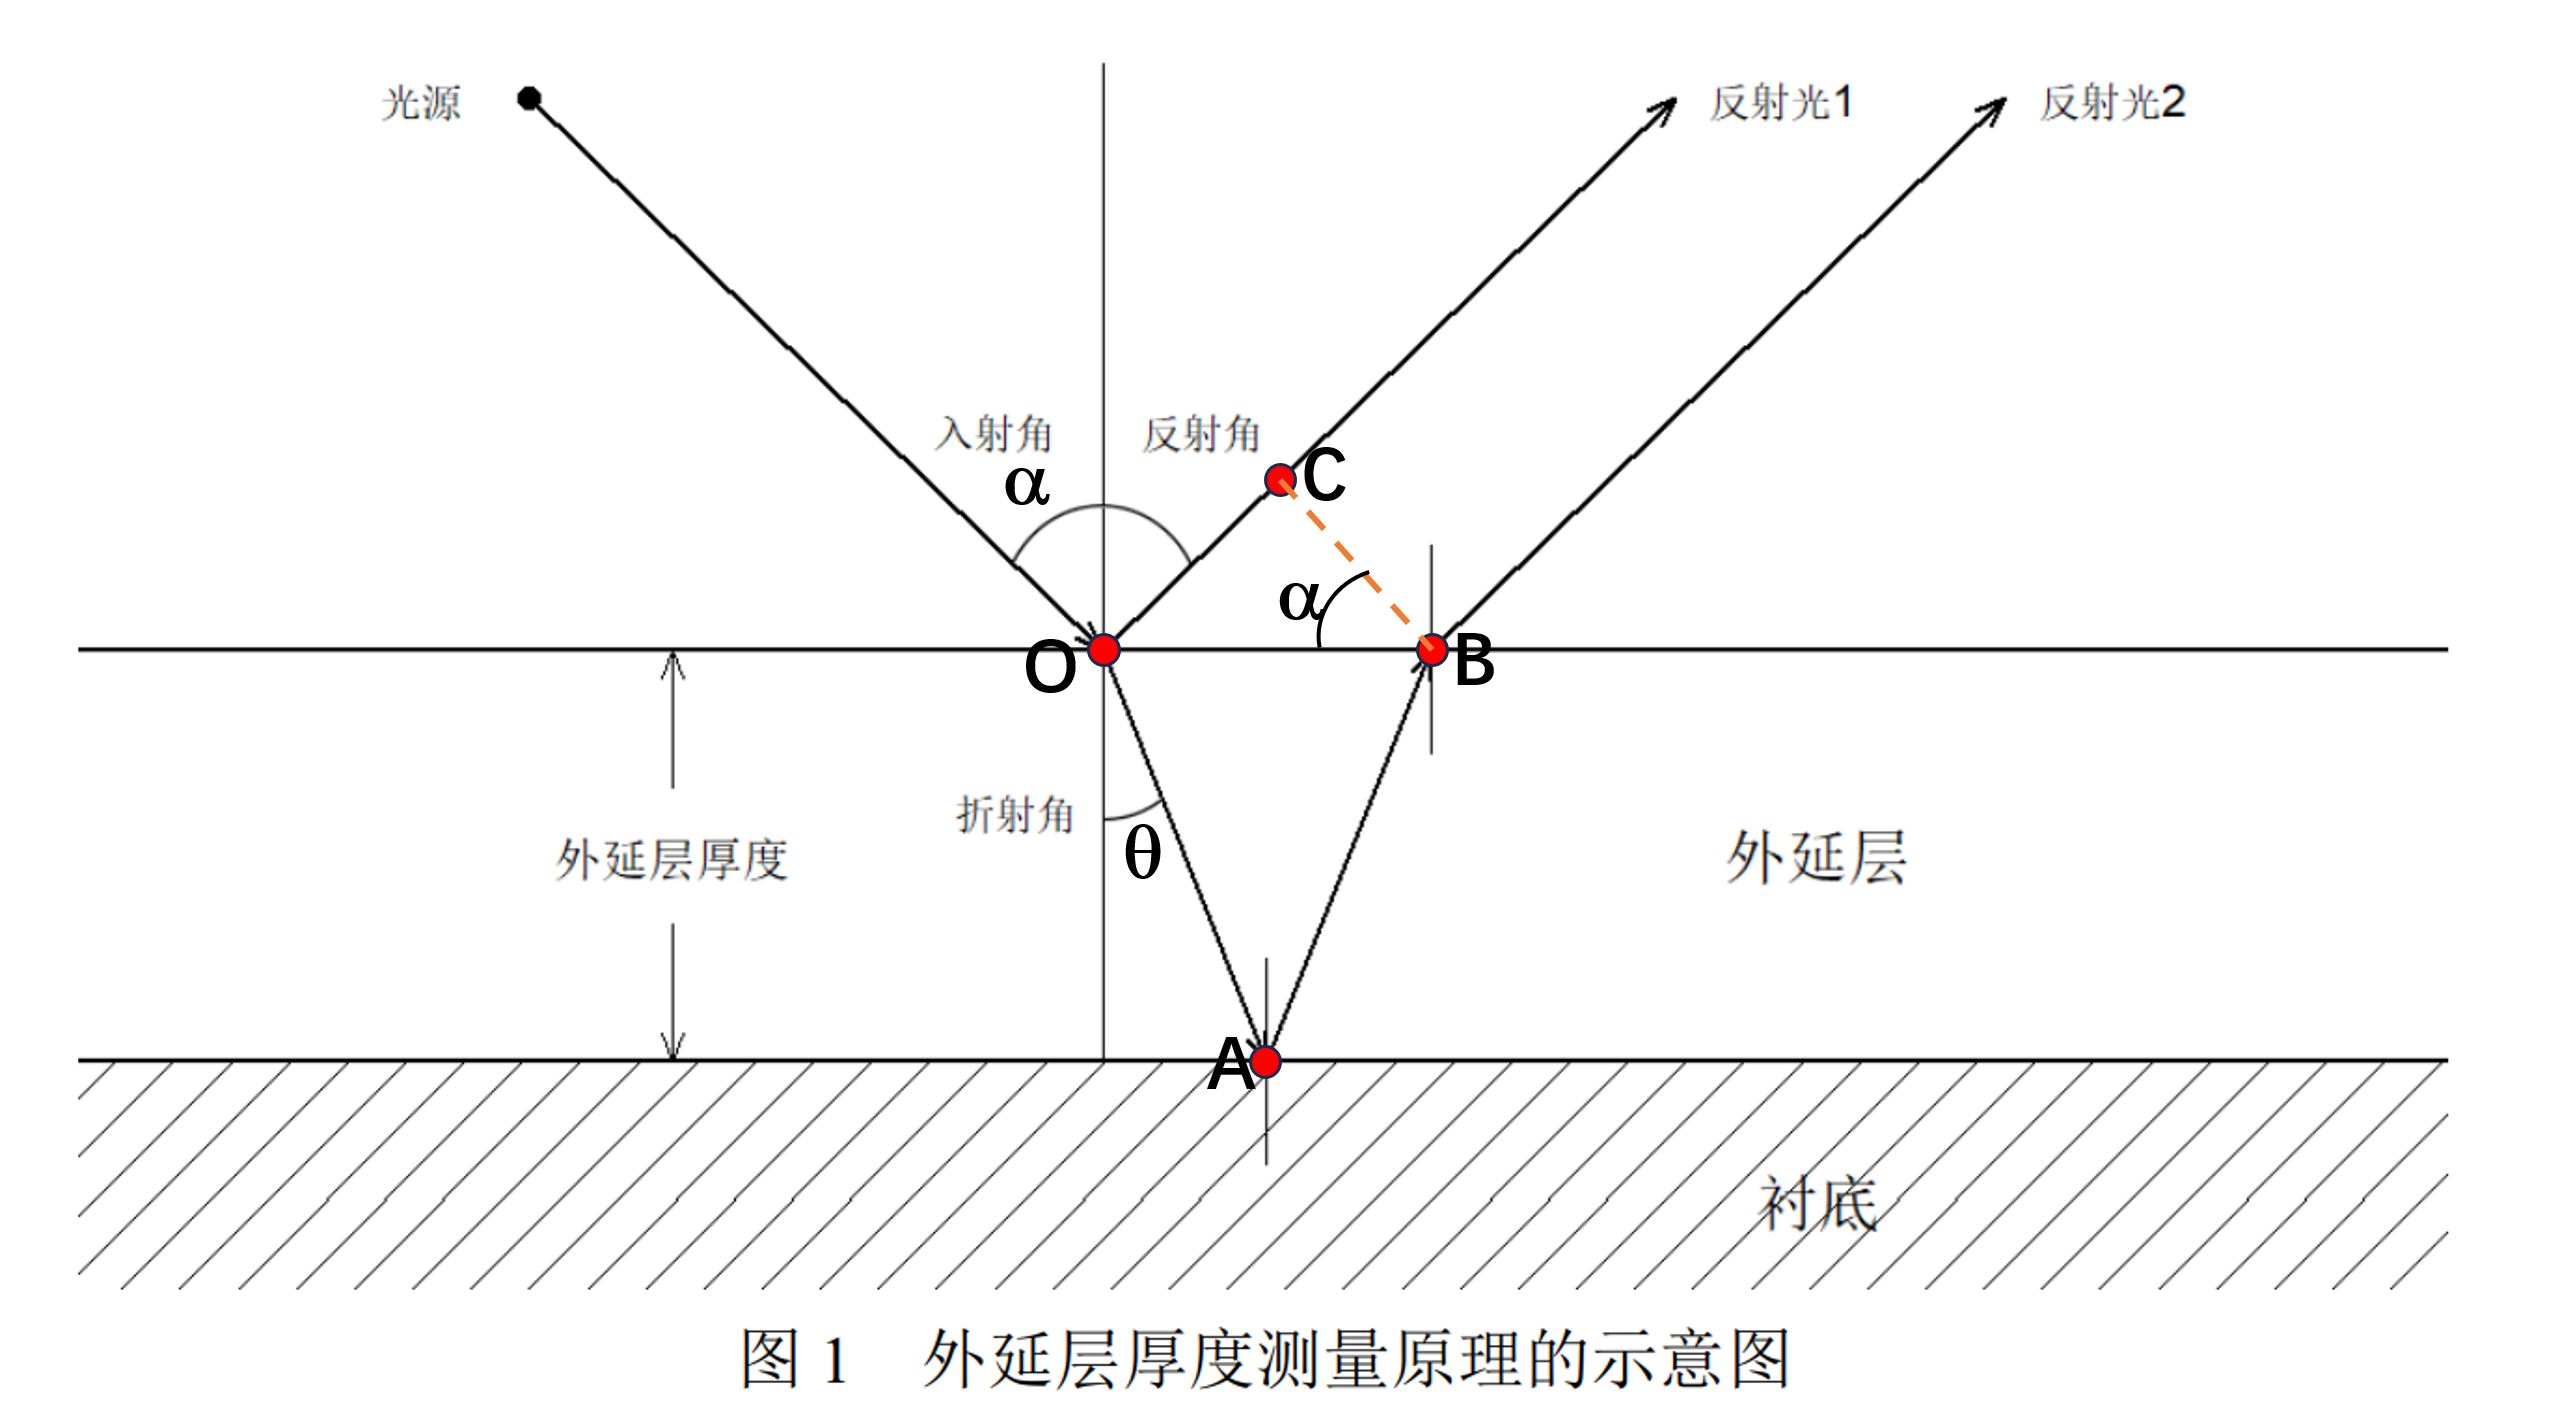
\includegraphics[width=0.8\textwidth]{q1_1.png}
	\caption{}
	\label{fig:q1_1}
	\end{figure}
考虑如图所示的双光束干涉几何结构,设入射光在介质界面发生折射后,形成两束相干光:一束经上表面反射(光程记为 $L_1$),另一束经下表面反射后返回(光程记为 $L_2$)。两束光在空气中叠加产生干涉条纹。根据几何关系,可得光程差 $\Delta L = L_2 - L_1$ 满足:

\begin{equation}
\Delta L = n_2 \cdot (AO + AB) - n_1 \cdot OC 
\end{equation}

其中:

\begin{itemize}
    \item $n_1$:入射介质(如空气)的折射率;
    \item $n_2$:外延层(如 SiC)的折射率;
    \item $d$:外延层厚度;
    \item $\alpha$:入射角(空气中);
    \item $\theta$:折射角(外延层内);
\end{itemize}
由几何对称性及折射定律,进一步可得:

\begin{align*}
AB &= AO = \frac{d}{n_2 \sin \theta}  \\
OC &= OB \cdot \tan \alpha = 2 \cdot AO \cdot \sin \theta \cdot \tan \alpha = 2d \cdot \frac{\tan \alpha}{n_2} 
\end{align*}
由于斯涅尔折射定律:
\begin{gather}
n_1 \sin \alpha = n_2 \sin \theta 
\end{gather}
联立(1)(2)(3)(4),并代入 $\tan \alpha = \frac{\sin \alpha}{\cos \alpha}$,解得:
\begin{align*}
\Delta L &= 2d \left( \frac{1}{\sin \theta} - \frac{n_1 \sin \alpha}{n_2 \cos \alpha} \right) \\
&= 2d \left( \frac{n_2}{n_1 \sin \alpha} - \frac{n_1 \sin \alpha}{n_2 \cos \alpha} \right) \quad \text{(代入 $\sin \theta$)}
\end{align*}

由于 $n_1 \approx 1$(空气),该式可进一步简化为:

\begin{equation}
\Delta L = 2d \sqrt{n_2^2 - \sin^2 \alpha}
\end{equation}
相位差:
\begin{gather}
	\Delta \phi = 2\pi \frac{\Delta L}{\lambda}
\end{gather}
干涉相长-“明纹”情况下双光束的相位差所满足的条件:
\begin{gather}
	\frac{2\pi}{\lambda}\Delta L = 2\cdot m\cdot \pi  \quad (m=1,2,3,\ldots)
\end{gather}
干涉相消-“暗纹”情况下双光束的相位差所满足的条件:
\begin{gather}
	\frac{2\pi}{\lambda}\Delta L = (2\cdot m + 1 )\cdot \pi \quad (m=1,2,3,\ldots)
\end{gather}
在实际观测中,我们发现SiC外延层的折射率会随着波长的变化而变化,在第二问的求解中,我们将会考虑波长对于折射率的影响。在此处,我们认为在波数变化极小的一段范围内,折射率可以视为常数。因此我们的结论是(带初相位$\varphi$):
\begin{equation}
	d = \frac{m (\lambda + \varphi)  }{2\sqrt{n_2^2 - \sin \alpha^2}}
\end{equation}
通过观测数据的两个峰值的间距,或者波谷(把波长换算为波数)。有:
\begin{equation}
2v_1d\sqrt{n_2^2 - \sin \alpha^2} = m
\end{equation}
\begin{equation}
2v_2d\sqrt{n_2^2 - \sin \alpha^2} = m+1
\end{equation}
(9)(10)作差得:
\begin{equation}
2(v_2-v_1)d\sqrt{n_2^2 - \sin \alpha^2} = 1
\end{equation}
令$
|v_1 - v_2| = \Delta T
$
,并整理得到外延层厚度d的表达式为:\begin{equation}
d = \frac{1}{2 \Delta T \sqrt{n_2^2 - \sin \alpha^2}}
\end{equation}
综上所述:厚度d由波数差$\Delta T$,折射率$n_2$,以及入射角$\alpha$确定,三者关系如下:
\begin{equation}
\begin{cases}
d = \dfrac{1}{2 \Delta T \sqrt{n_2^{2}-\sin^{2}\theta}}\\[4pt]
|v_{1}-v_{2}|=\Delta T\\[4pt]
n_{2}=f(v)
\end{cases}
\label{eq:thickness}
\end{equation}
其中$f(v)$为波数与折射率的关系函数,该函数与材料本身性质有关。
	\section{第二问的模型的建立和求解}
	由第一问可以得到厚度计算的基本模型,针对给出的SiC材料红外干涉法的数据,我们将通过数据预处理、折射率函数求解、周期提取、模型验证等步骤,应用第(1)问的模型并求解。
	\begin{figure}[H]
	\centering
	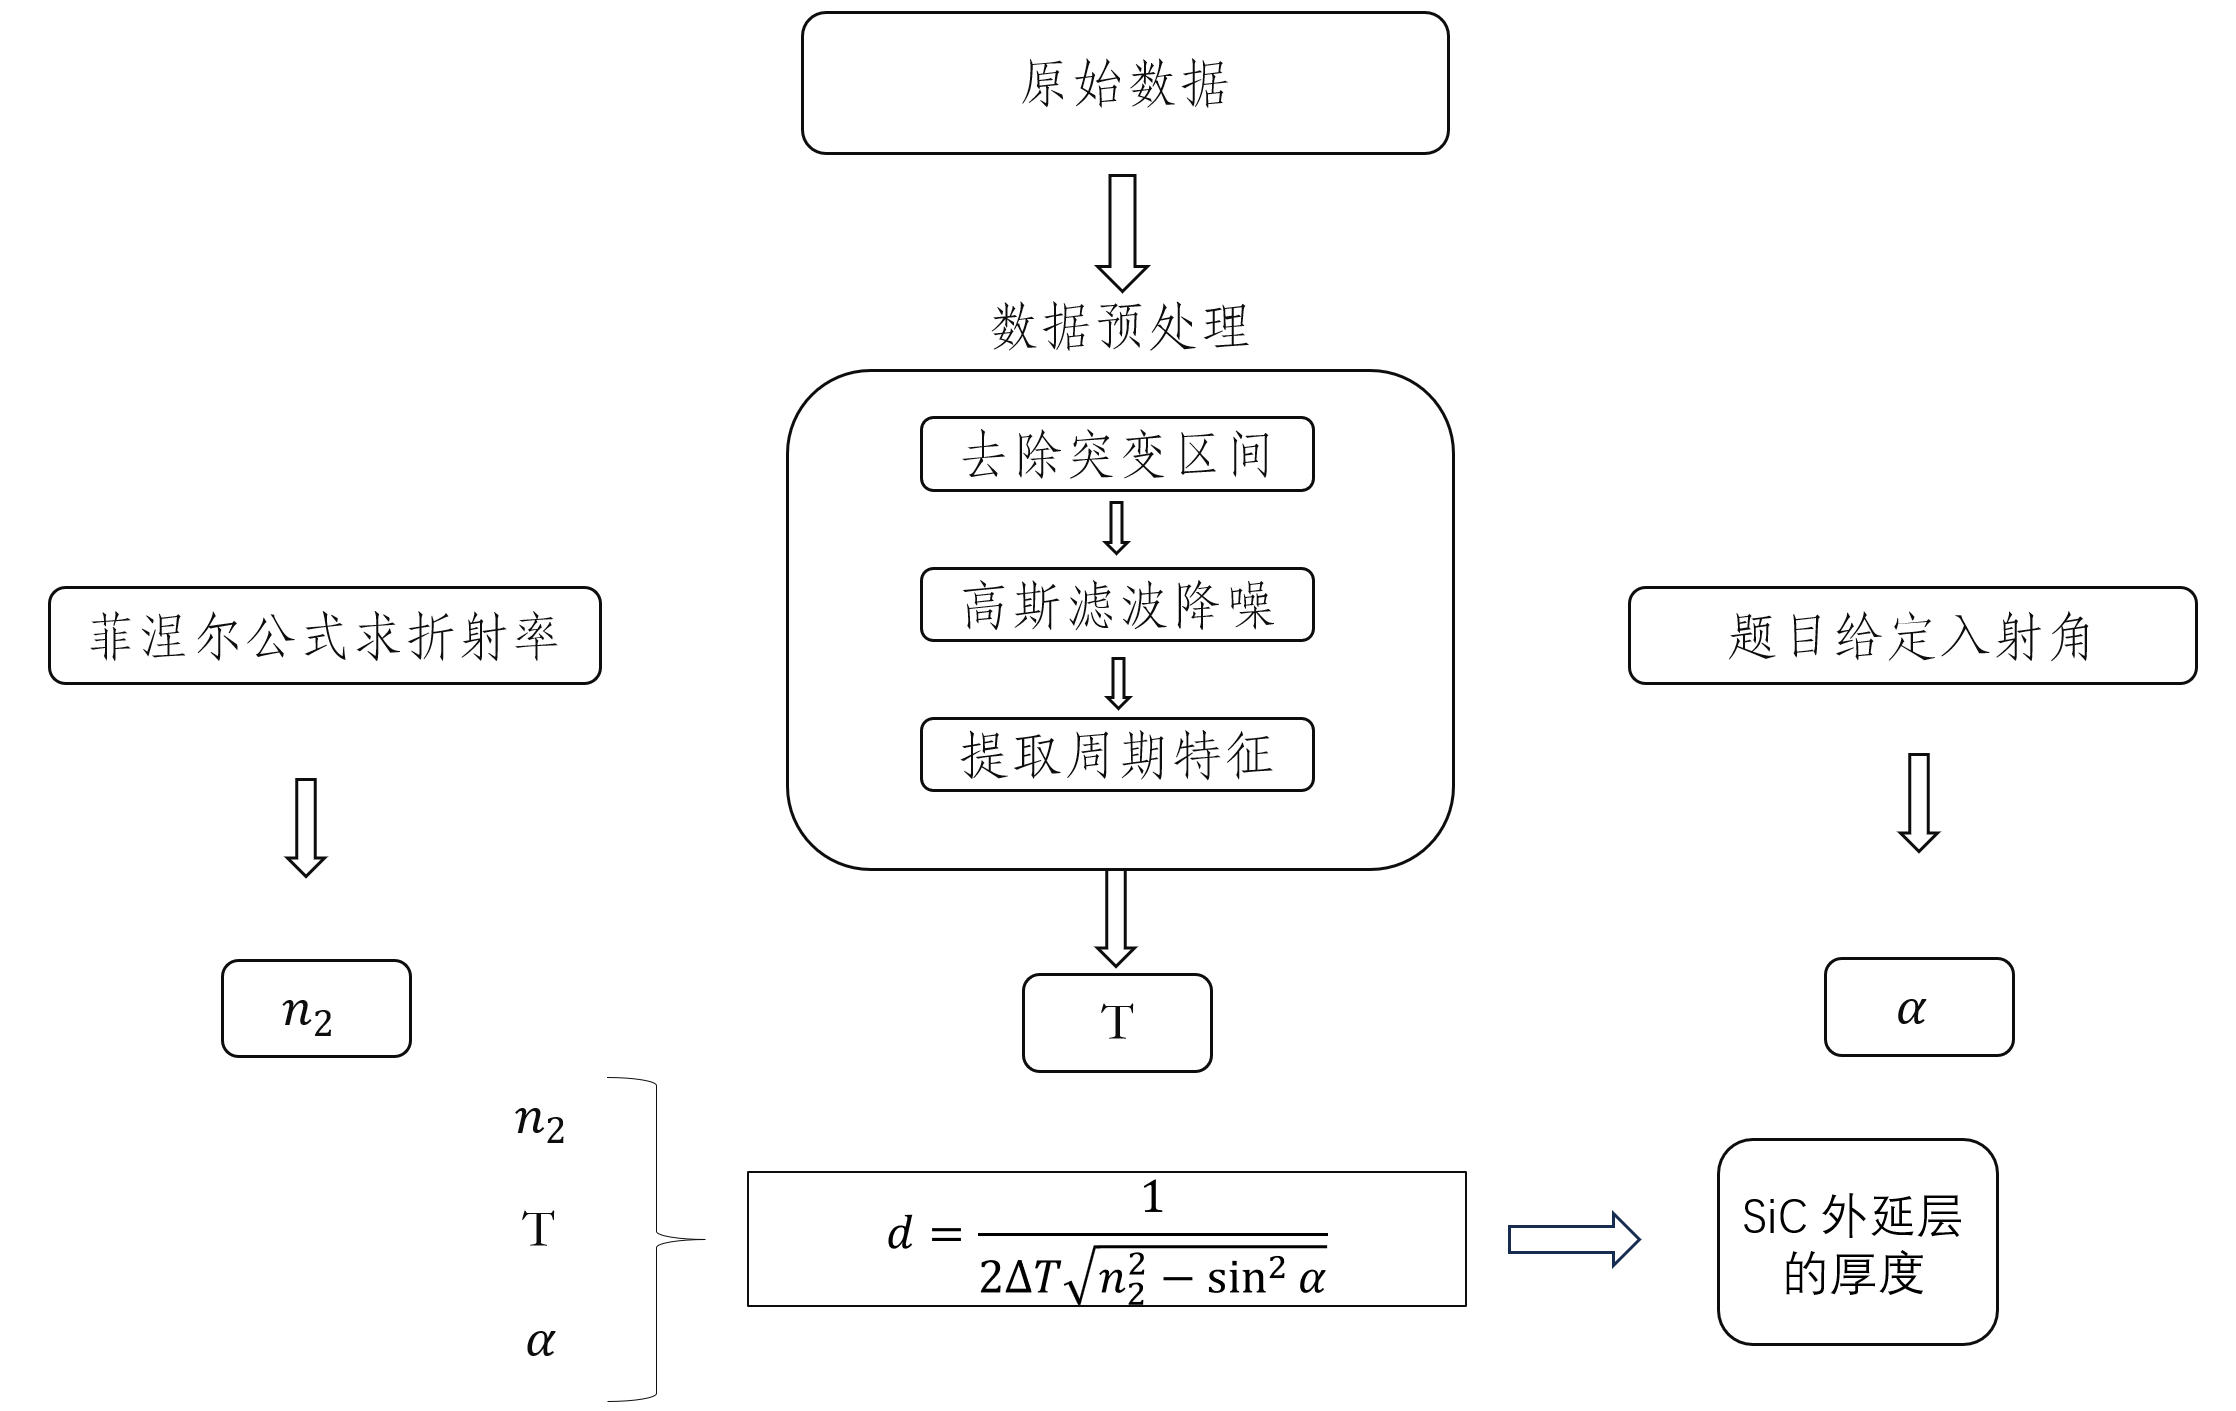
\includegraphics[width=.97\linewidth]{微信图片_20250907180628_10527_543.png}
	\caption{流程图}
	\label{流程图}
	\end{figure}
	\subsection{数据可视化与预处理}
	\begin{figure}[H]
	\centering
	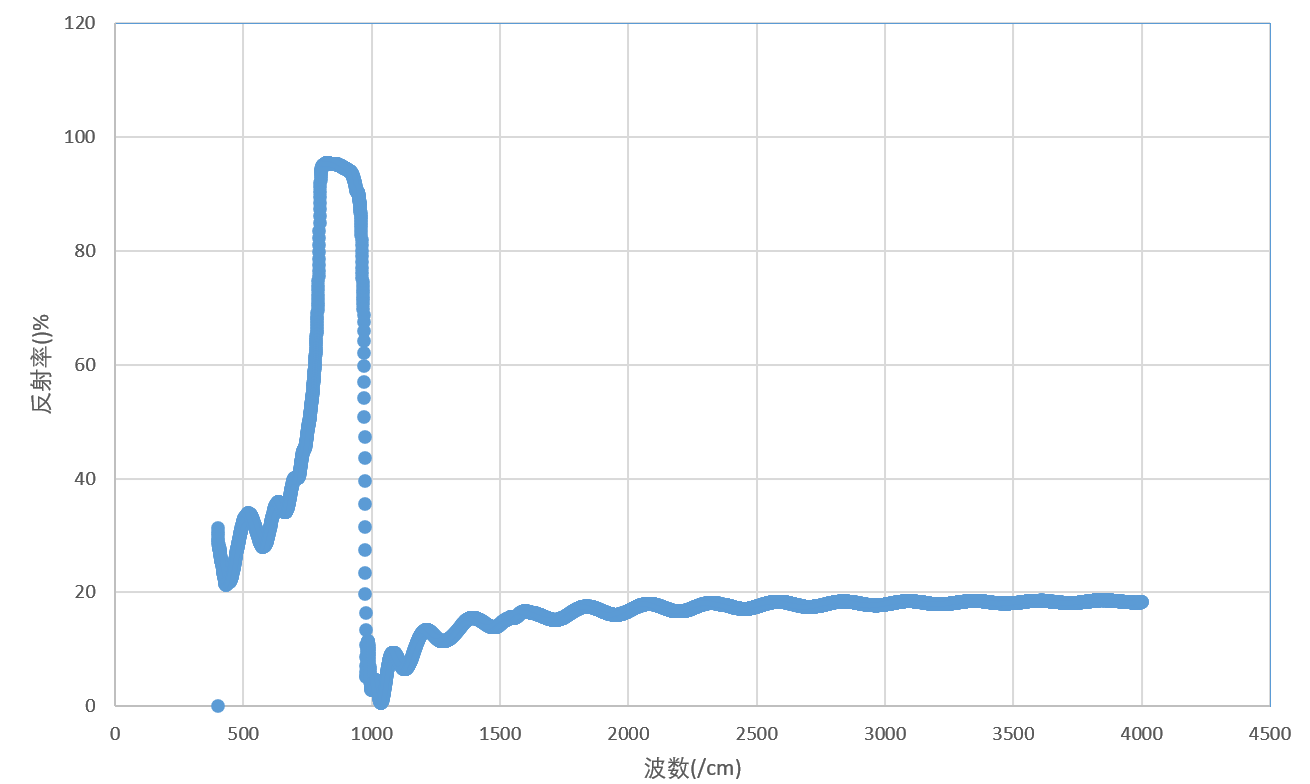
\includegraphics[width=.6\linewidth]{屏幕截图 2025-09-07 115010.png}
	\caption{附件1 反射率-波数图}
	\label{fig:refraction_process}
	\end{figure}
	绘制附件一的图像,我们明显看到,附件1数据在波数在500-1000cm$^{-1}$范围有着明显的突变,附件2的数据特征与之类似。通过查询论文\upcite{Najbauer2024Uncovering},我们得知, SiC 外延样品的反射光谱可分为四个光谱区域,

	\begin{itemize}
  \item 500–700 cm$^{-1}$:厚度振荡区,对材料本身杂志等成分敏感;
  \item 700–1000 cm$^{-1}$:余辉带,具有高吸收率;
  \item 1000–1500 cm$^{-1}$:过渡区,介于吸收与透明之间;
  \item $>1500$ cm$^{-1}$:透明区,能够较好的显示厚度产生的振荡。
\end{itemize}
	因此,我们选取波数在1500 cm$^{-1}$以上的数据进行分析。
已知入射角为 $\theta_i$,反射光与折射光的光强比为 $K=\dfrac{I_r}{I_t}$,入射介质折射率为 $n_1$(通常取空气 $n_1\approx 1$)。为求未知介质折射率 $n_2$,首先将强度比转化为总反射率 $R$:

\begin{equation}
R=\frac{K}{K+1}.
\end{equation}
随后,采用高斯滤波器对原始反射率–波数数据进行降噪处理,以消除高频噪声并获取平滑、可解析的光谱曲线。
\subsubsection{菲涅尔公式}
	外延层的折射率通常不是常数,它与掺杂载流子的浓度、红外光谱的波长等参数有关。由于附件1和附件2使用的是同一块块碳化硅晶圆片,故可以假设载流子浓度一定,折射率仅与波长有关。
	
	菲涅耳公式描述了光在不同介质分界面上的反射和折射的振幅、相位等关系。能够结合光的反射、折射等光学现象的观测数据来得到折射红外光谱的波长等参数有关。
	这两个公式给出了 $R_s$ 和 $R_p$ 的具体表达式。

\begin{itemize}
    \item s-偏振反射率 ($R_s$):
    \[
    R_s = \left| \frac{n_1 \cos \theta_i - n_2 \cos \theta_t}{n_1 \cos \theta_i + n_2 \cos \theta_t} \right|^2
    \]
    
    \item p-偏振反射率 ($R_p$):
    \[
    R_p = \left| \frac{n_2 \cos \theta_i - n_1 \cos \theta_t}{n_2 \cos \theta_i + n_1 \cos \theta_t} \right|^2
    \]
\end{itemize}
其中,$n_1$为入射介质的折射率,$n_2$为折射介质的折射率,$\theta_i$为入射角度,$\theta_t$为折射角度。
$R_s$和$R_p$分别是s-偏振光 (TE波)和p-偏振光 (TM波)的表达式。我们认为,红外干涉法所使用的光为非偏振光,反射率$R = \frac{1}{2}(R_s + R_p)$。

与式(2)进行联立,我们解得:
	\begin{equation}
	\begin{split}
	R = \frac{K}{K + 1} = &\frac{1}{2}\bigg[ \left( \frac{n_1 \cos\theta_i - \sqrt{n_2^2 - n_1^2 \sin^2\theta_i}}{n_1 \cos\theta_i + \sqrt{n_2^2 - n_1^2 \sin^2\theta_i}} \right)^2 + \\
	&\left( \frac{n_2^2 \cos\theta_i - n_1 \sqrt{n_2^2 - n_1^2 \sin^2\theta_i}}{n_2^2 \cos\theta_i + n_1 \sqrt{n_2^2 - n_1^2 \sin^2\theta_i}} \right)^2 \bigg]
	\end{split}
	\end{equation}
\subsubsection{计算折射率}
上文提到,波数在1500cm$^{-1}$以上时,SiC可视为透明介质,即光线射向SiC表面时只会发生反射、透射而不会吸收。又由于本题的假设中,仅考虑双光束干涉,所以我们认为在双光束干涉近似下,透明介质(如SiC,无吸收)薄膜的反射率由两束相干光叠加决定:第一束为上表面直接反射光,其强度 $ R_0 $ 依赖入射角 $ \theta_0 $,取式(14)菲涅尔反射率 $ R_0 $,其中 $ \theta $ 为膜内折射角,满足 式(2)$ n_0 \sin\theta_0 = n \sin\theta $;第二束光强度为 $ R_1 = R_0 (1 - R_0)^2 $。二者相位差为 $ \phi = \frac{4\pi}{\lambda} n d \cos\theta $。总反射率为:
\begin{equation}
R = R_0 + R_1 - 2\sqrt{R_0 R_1} \cos\phi
\end{equation}
反射率随 $ d $、$ \lambda $ 或 $ \theta_0 $ 呈周期性变化。
观察式(15),我们发现SiC外延层反射率随波数变化的图象可进行分解为两个部分:第一部分是与波数无关的常数项,第二部分是与波数相关的项。
利用傅里叶变换,我们将附件1、2的数据分解为了波动部分和趋势部分,如图所示:
\begin{figure}[H]
  \centering
  \begin{subfigure}[b]{0.49\linewidth}
    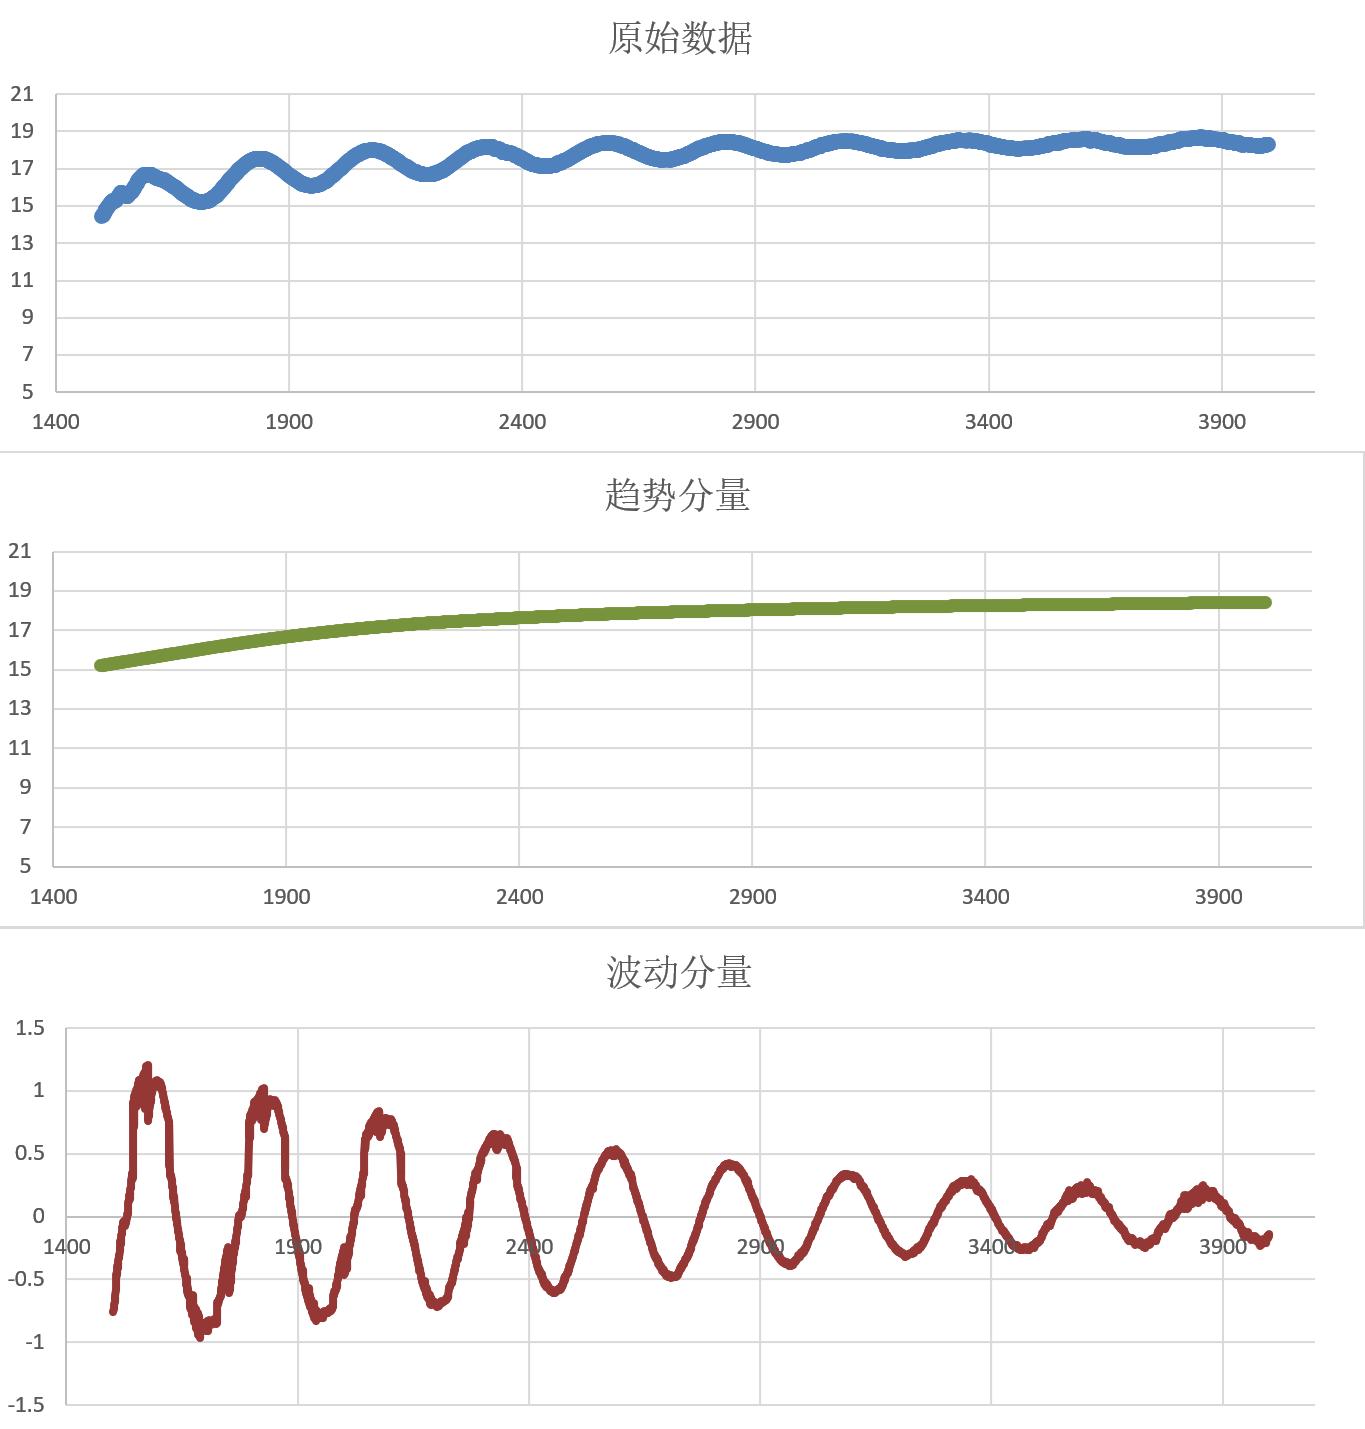
\includegraphics[width=\linewidth]{屏幕截图 2025-09-07 130331.png}
    \caption{附件1 趋势-波动示意图}
    \label{fig:att1}
  \end{subfigure}
  \hfill
  \begin{subfigure}[b]{0.49\linewidth}
    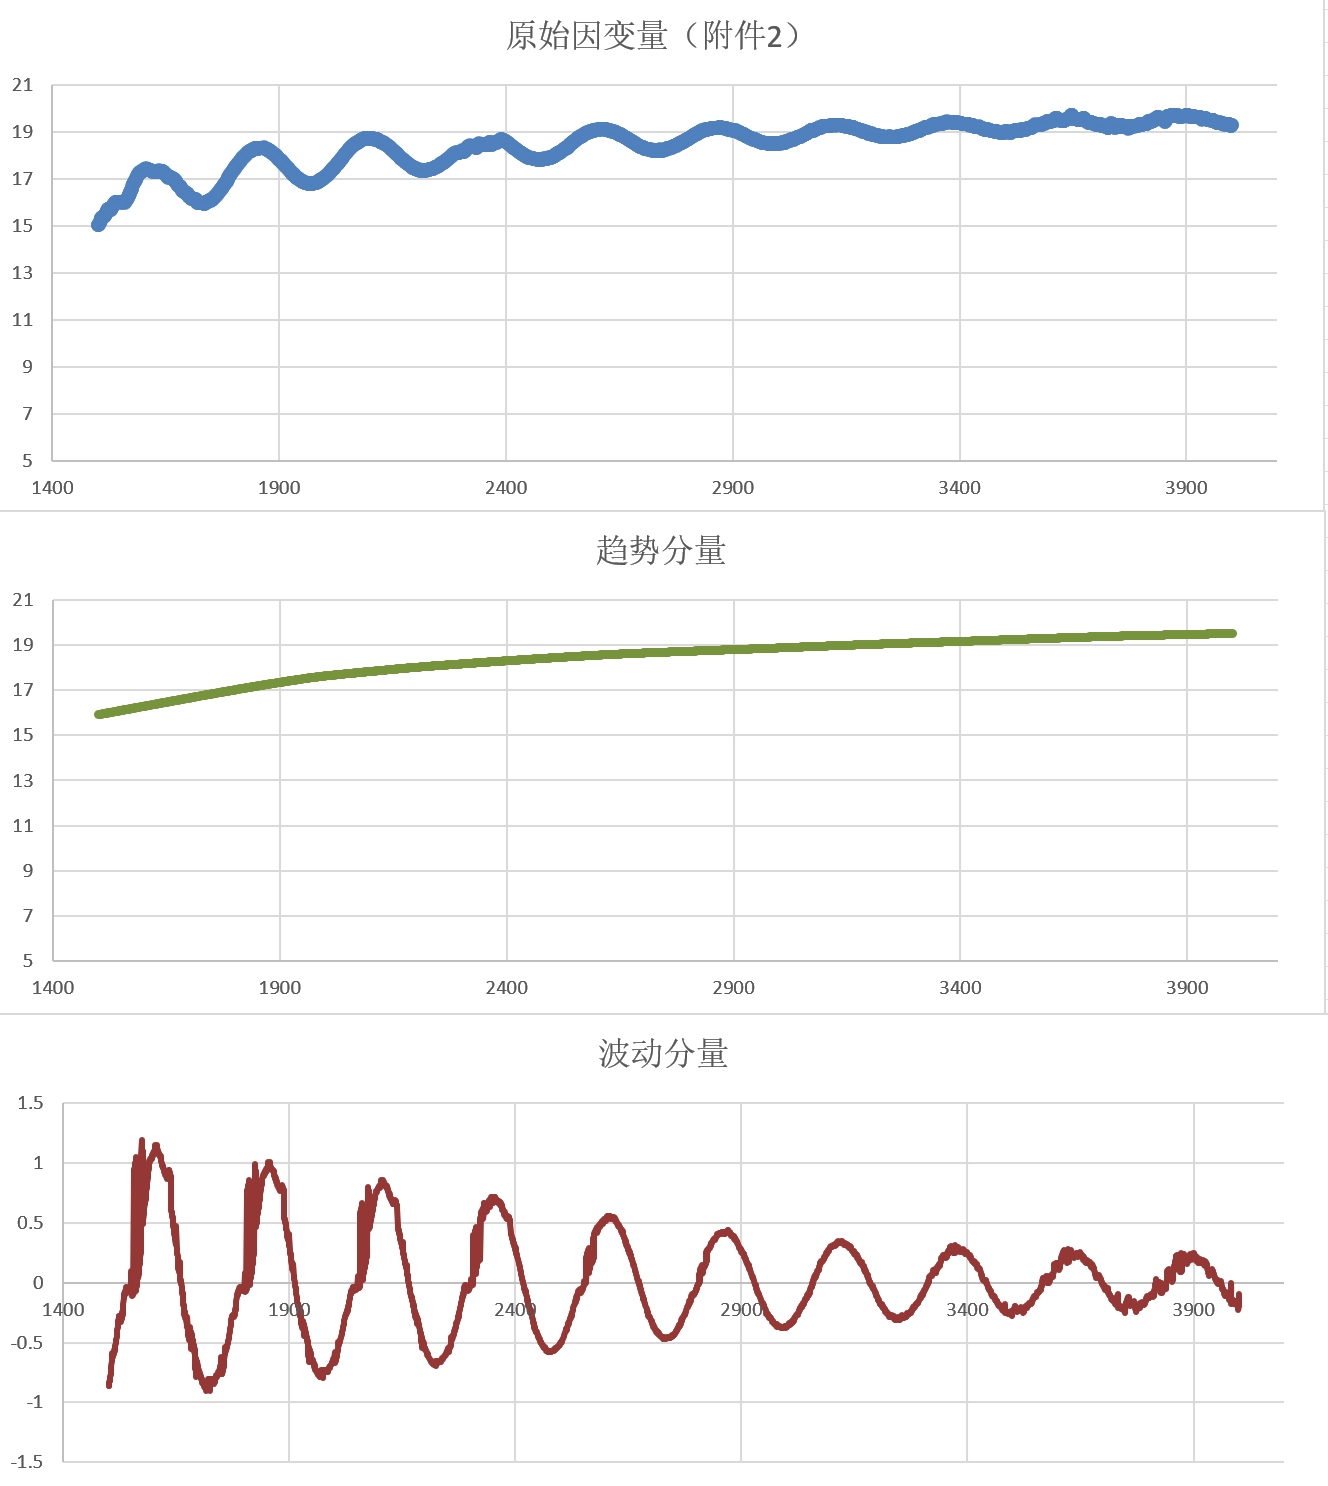
\includegraphics[width=\linewidth]{屏幕截图 2025-09-07 130757.png}
    \caption{附件2 趋势-波动示意图}
    \label{fig:att2}
  \end{subfigure}
  \caption{}
  \label{fig:double}
\end{figure}
图中趋势部分的大小代表$R_0+R_1$的大小,波动部分的振幅代表$2\sqrt{R_0 R_1}$的大小。
对范围内的$R_0$和$R_1$进行求解,我们可以得到$R_0$随波束变化的函数图象,如图所示:
\begin{figure}[H]
  \centering
  \begin{subfigure}[b]{0.45\linewidth}
    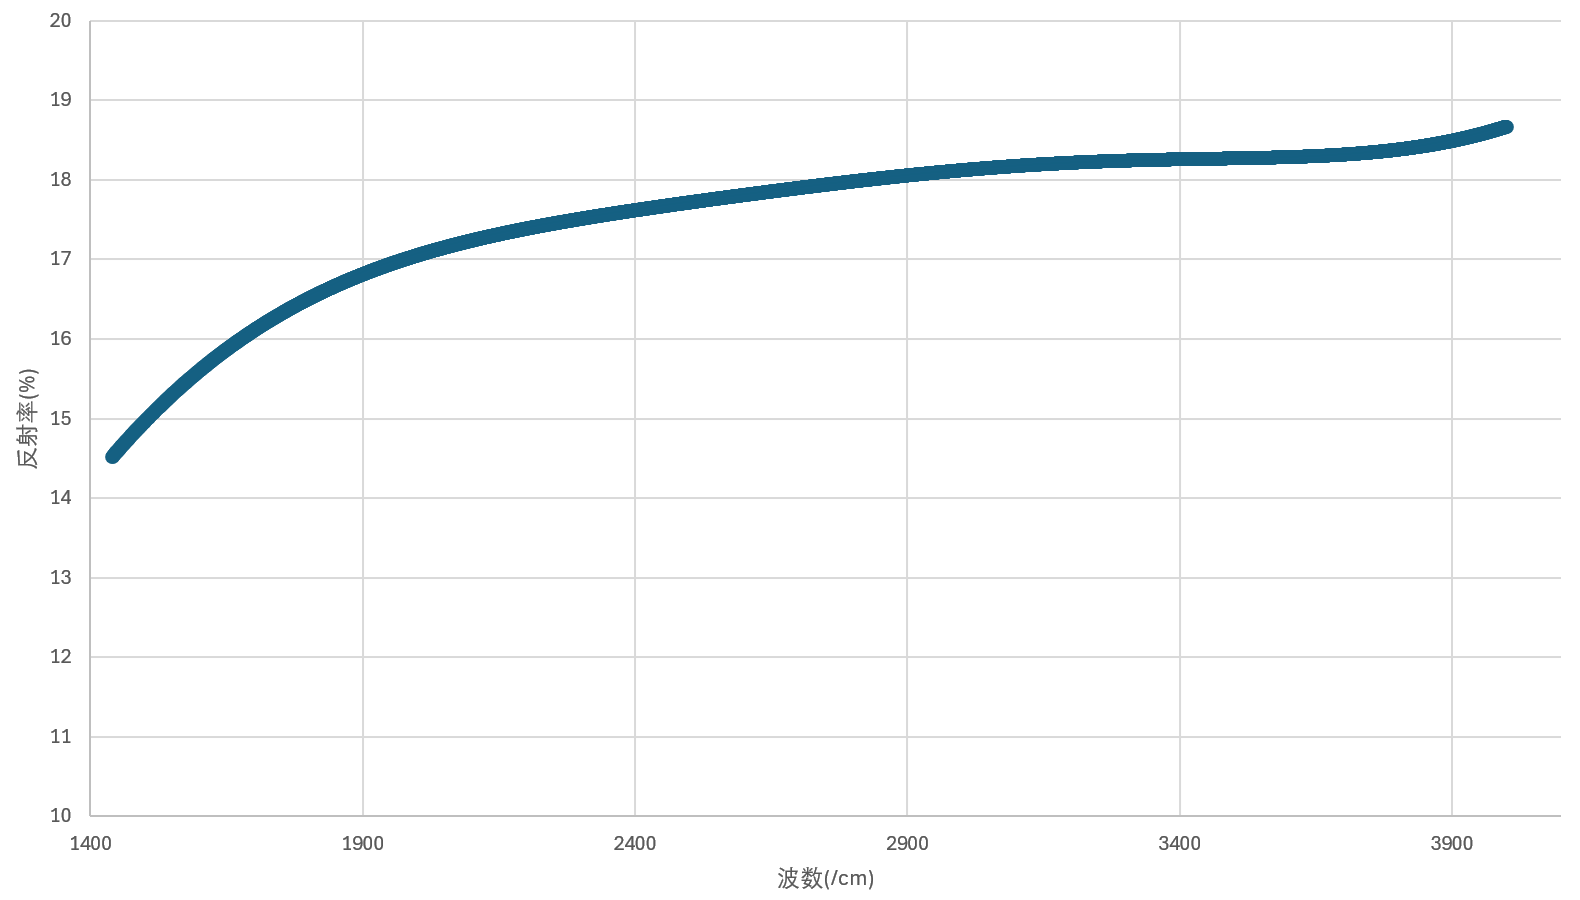
\includegraphics[width=\linewidth]{屏幕截图 2025-09-07 132303.png}

    \caption{附件1 反射率数据}
    \label{fig:附件1 反射率数据}
  \end{subfigure}
  \hfill
  \begin{subfigure}[b]{0.45\linewidth}
    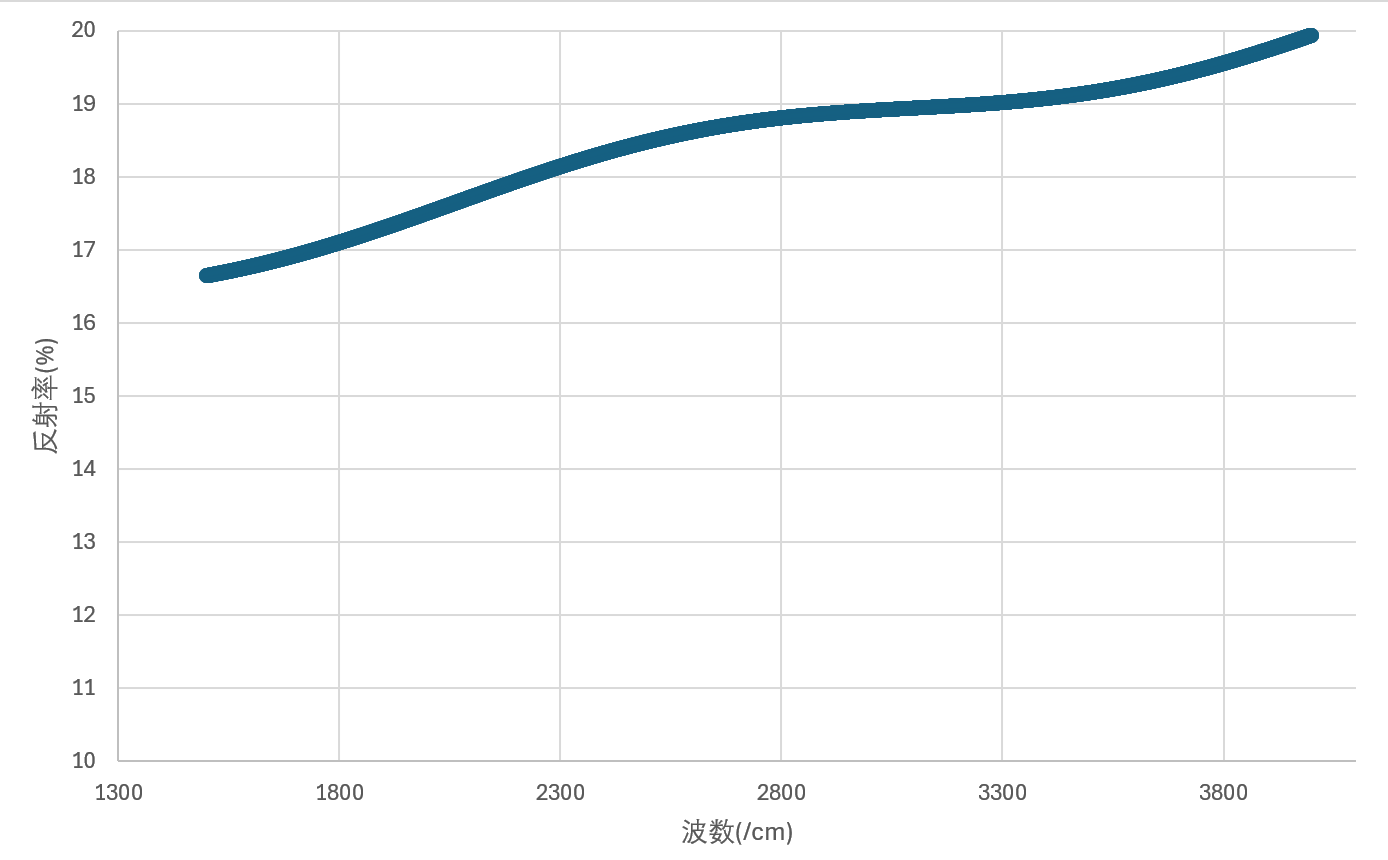
\includegraphics[width=\linewidth]{屏幕截图 2025-09-07 132440.png}
    \caption{附件2 反射率数据}
    \label{fig:附件2 反射率数据}
  \end{subfigure}
  \caption{}
  \label{fig:double2}
\end{figure}
接着,分别在10°(附件1)和15°(附件2)的情境下代入式(14)求得数值解,如图,以下是附件1和附件2的折射率计算结果:
\begin{figure}[H]
  \centering
  \begin{subfigure}[b]{0.49\linewidth}
    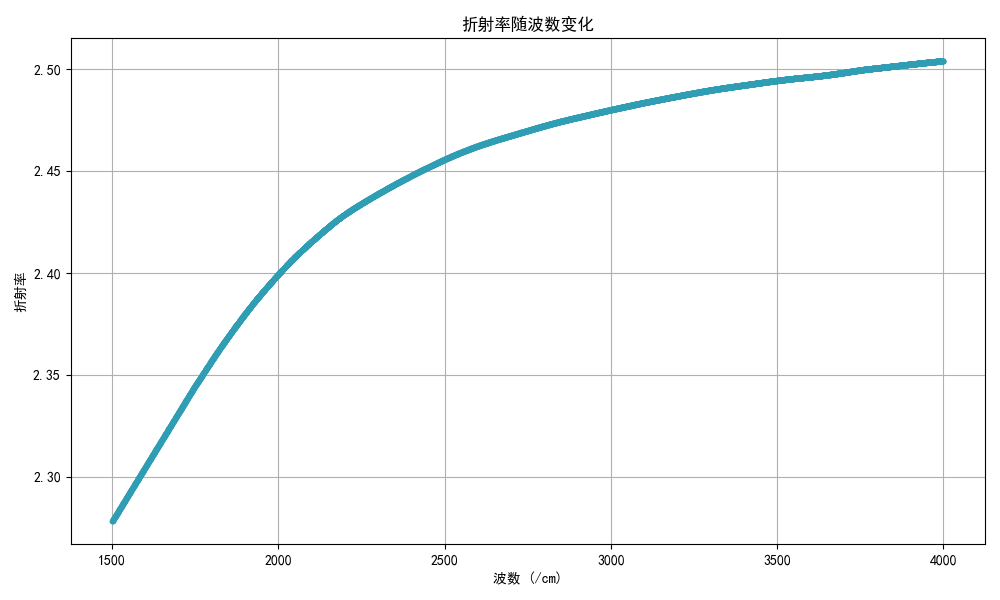
\includegraphics[width=\linewidth]{新输出结果喵.png}

    \caption{附件1 折射率数据}
    \label{fig:附件1 反射率数据}
  \end{subfigure}
  \hfill
  \begin{subfigure}[b]{0.49\linewidth}
    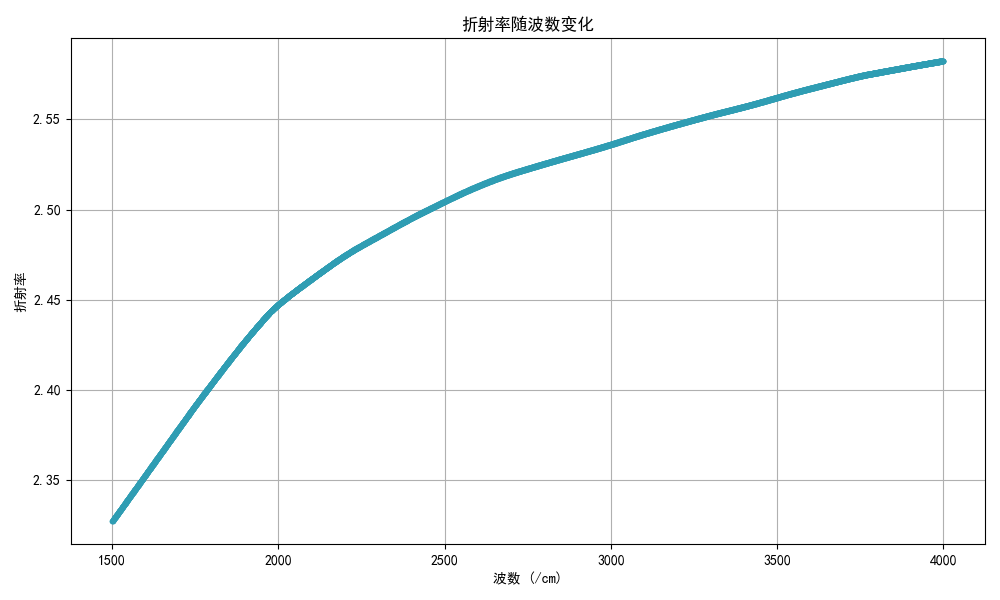
\includegraphics[width=\linewidth]{新输出结果2喵.png}
    \caption{附件2 折射率数据}
    \label{fig:}
  \end{subfigure}
  \caption{}
  \label{fig:double3}
\end{figure}

\subsection{计算外延层厚度}
利用方程组(13)所代表的模型,我们将上述折射率函数代入,在附件1和附件2数据中分别取点进行计算。其中,附件1的数据平均值为7.5080,方差为0.000256;附件2的数据平均值为7.4837,方差为0.00133。
综上,SiC外延层的厚度为$7.4959\pm0.0307~\mu\mathrm{m}$。
\subsection{模型验证}
将两组数据进行对比,如图所示
\begin{figure}[H]
  \centering
  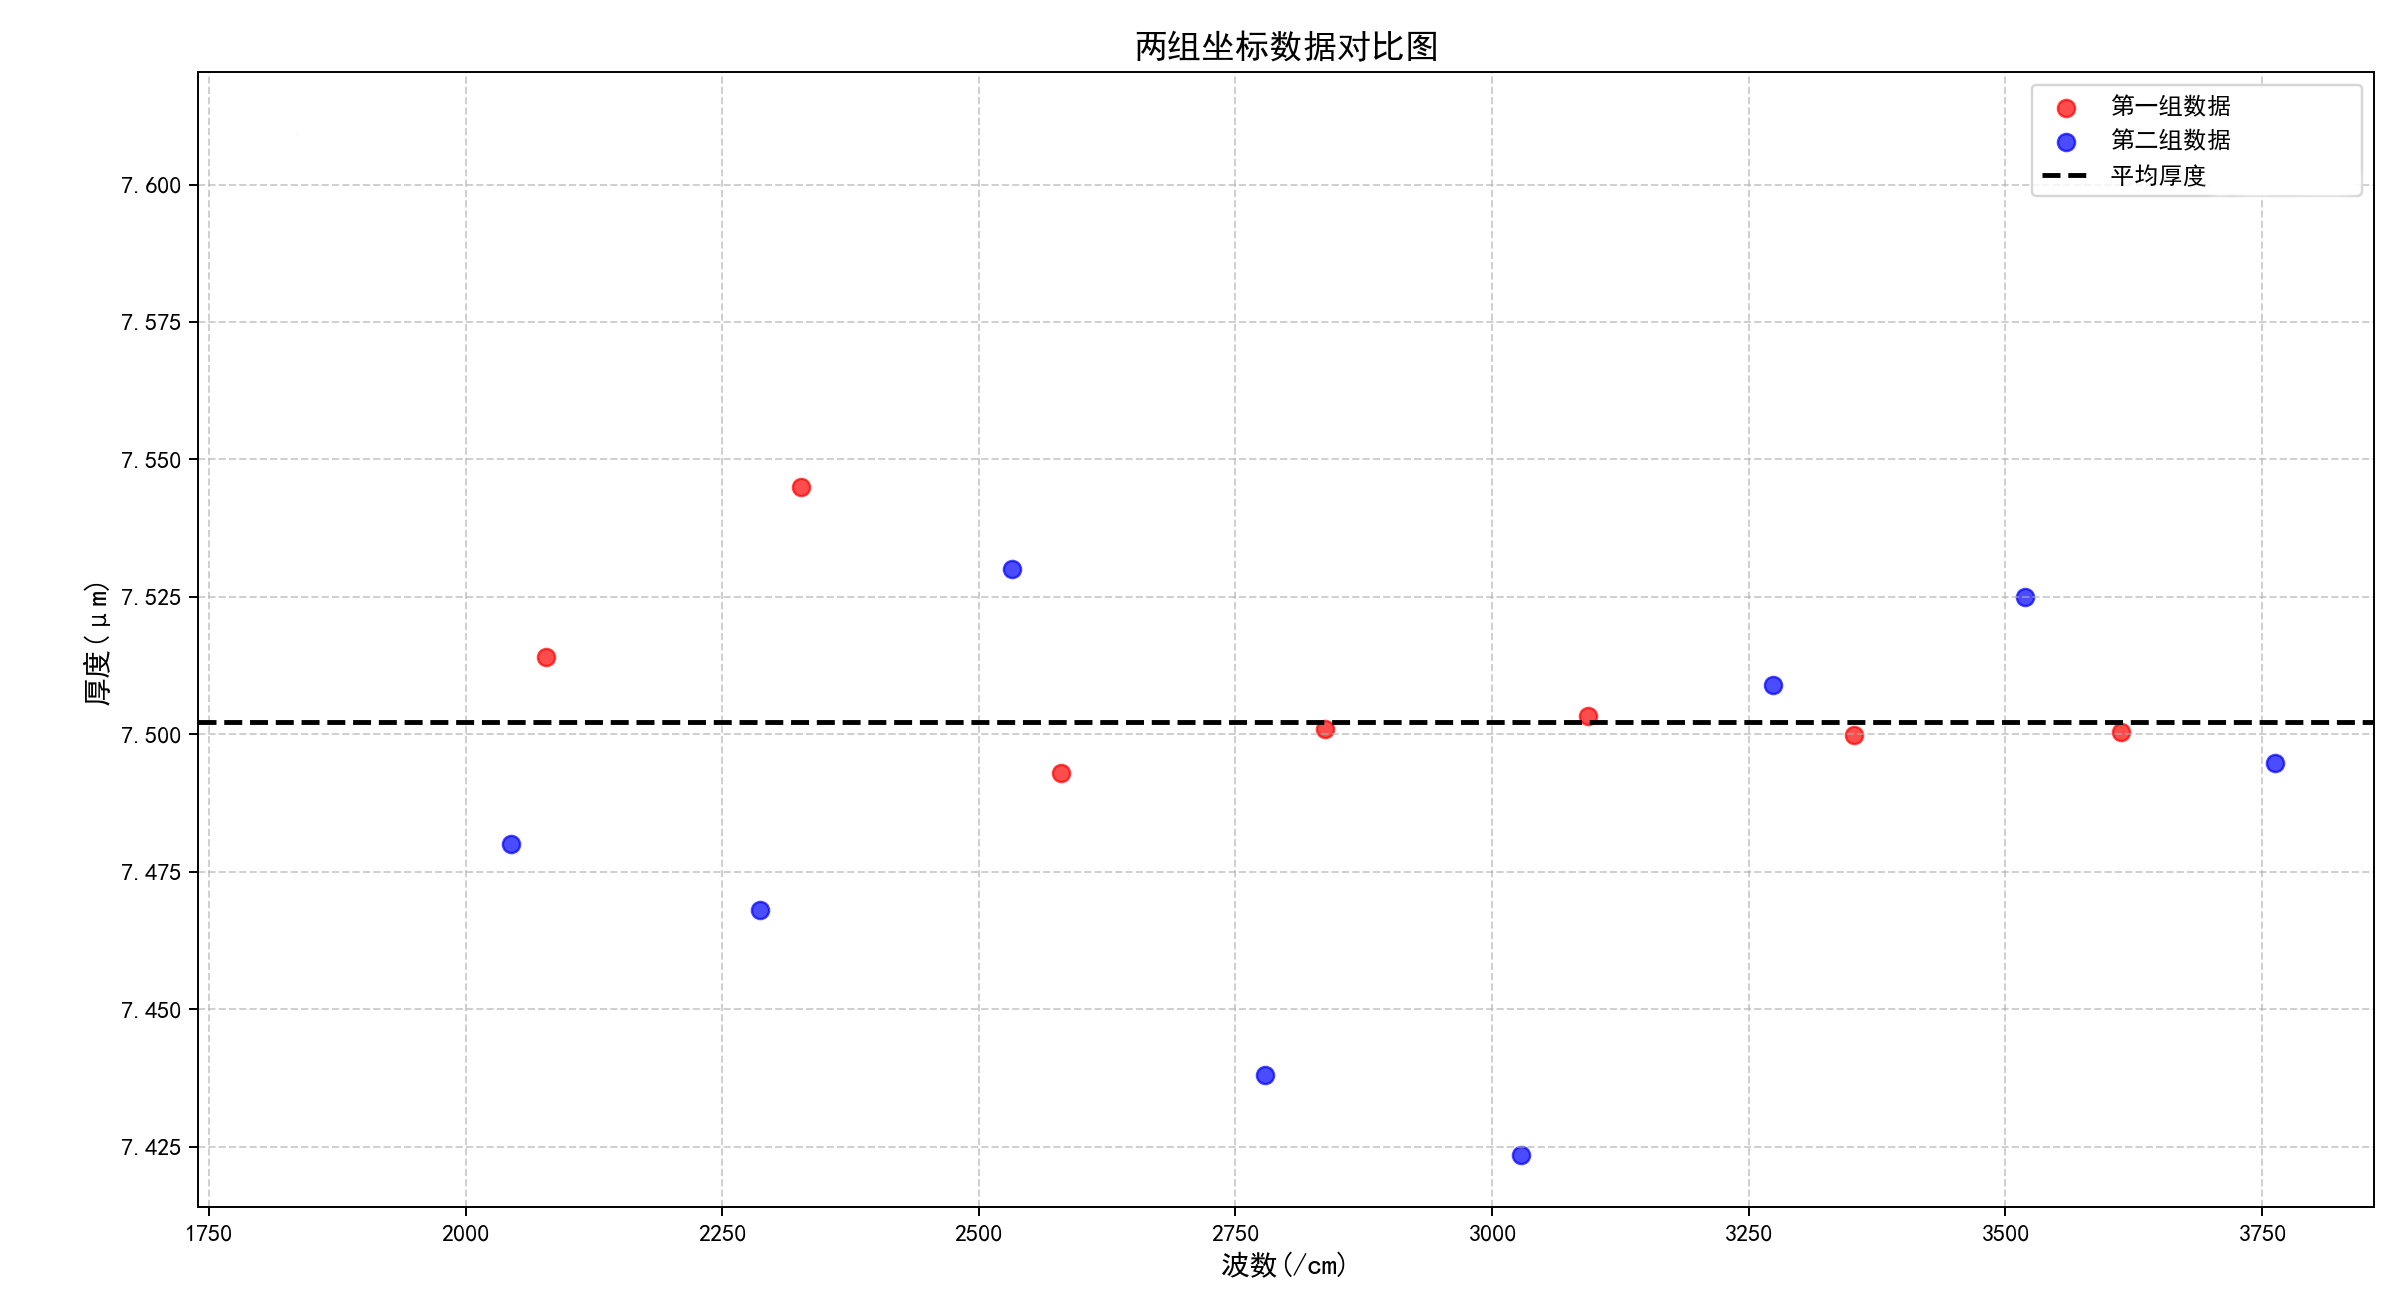
\includegraphics[width=.65\linewidth]{未标题-3.png}
  \caption{两组数据对比}
  \label{fig:untitled3}
\end{figure}
根据题设条件,附件一与附件二系基于同一块样品材料在不同入射角条件下所进行的两组独立实验。从物理原理出发,材料的特征参数 $ d $ 应在两次实验中保持一致。为验证模型的稳健性与一致性,本文采用与附件一相同的处理方法对附件二数据进行分析,独立求解其对应的 $ d $ 值,并进一步计算两组结果之间的相对偏差。若所得 $ d $ 值的相对偏差处于可接受误差范围内,则可认为所建立的模型具有良好的可靠性与重现性,从而支持其在实际应用中的有效性。

根据计算,两组厚度数据的差值仅为$0.024\mu\mathrm{m}$,方差为0.000941。该数据表明,基于不同入射角条件下获得的两组厚度测量结果具有高度一致性。考虑到实验测量中可能存在的仪器误差、环境扰动及数据拟合过程中的数值不确定性,偏差处于合理误差容限之内,佐证了模型在不同实验条件下的稳定性与鲁棒性。
\section{第三问模型分析与求解}

\subsection{必要条件}

\begin{enumerate}
	\item \textbf{时间相干性和空间相干性} 
	 
	从时间相干性分析,由于实际光源所发出的光波并非理想的无限长单色波列,而是具有一定持续时间的有限长波列,因此,当多束光参与干涉时,光源的相干长度必须大于多光束间的最大光程差,否则无法形成稳定的干涉现象。
	 从空间相干性角度分析,其核心是表征光源不同空间位置发出的光之间的相干特性,要求入射光束必须为平行光(即准直光)。若入射光为非平行光,会导致不同位置反射光的波前相位差产生随机波动,进而造成干涉条纹模糊,甚至无法形成有效的干涉现象。
	
	 为满足该条件,外延层需具备高度均匀的厚度和平整的表面,以确保各反射波前相位关系稳定;外延层应具有低散射、高透射/反射一致性,以维持入射平行光的波前完整性,从而保障空间相干性。同时,外延层的厚度应当在一定范围内,否则将无法满足时间相干性。
	
	\item \textbf{光波在外延层界面和衬底界面发生多次反射和透射}  \\
	光束在每一次界面反射的时候都会产生光强衰减,假设单次反射率为R,则经过i次反射后,反射光的相对光强需要乘$R^i$。如果R过低,两次或者多次反射光的光强会大幅度减小,以至于逐渐趋近于0,导致后面的光难以对两束反射光行成的干涉光产生影响,难以形成新的明显的多光干涉现象(此种情况属于退化为双光干涉)。
		 
	设介质外延层与空气界面处,由空气射入外延层的反射率为$r$,折射率为$t_1$,由外延层射向空气的折射率为$t_2$,外延层与衬底界面(由外延层射向衬底)的反射率为$r'$\\
	菲涅尔公式可以表示折射率与反射率的关系,我们由折射率推导出反射率(此处取垂直入射情况,作定性分析):
	$$R = \left( \frac{n_1 - n_2}{n_1 + n_2} \right)^2 $$
	根据能量守恒有:\[ R + T = 1 \]
	\begin{figure}[H]
		\centering
		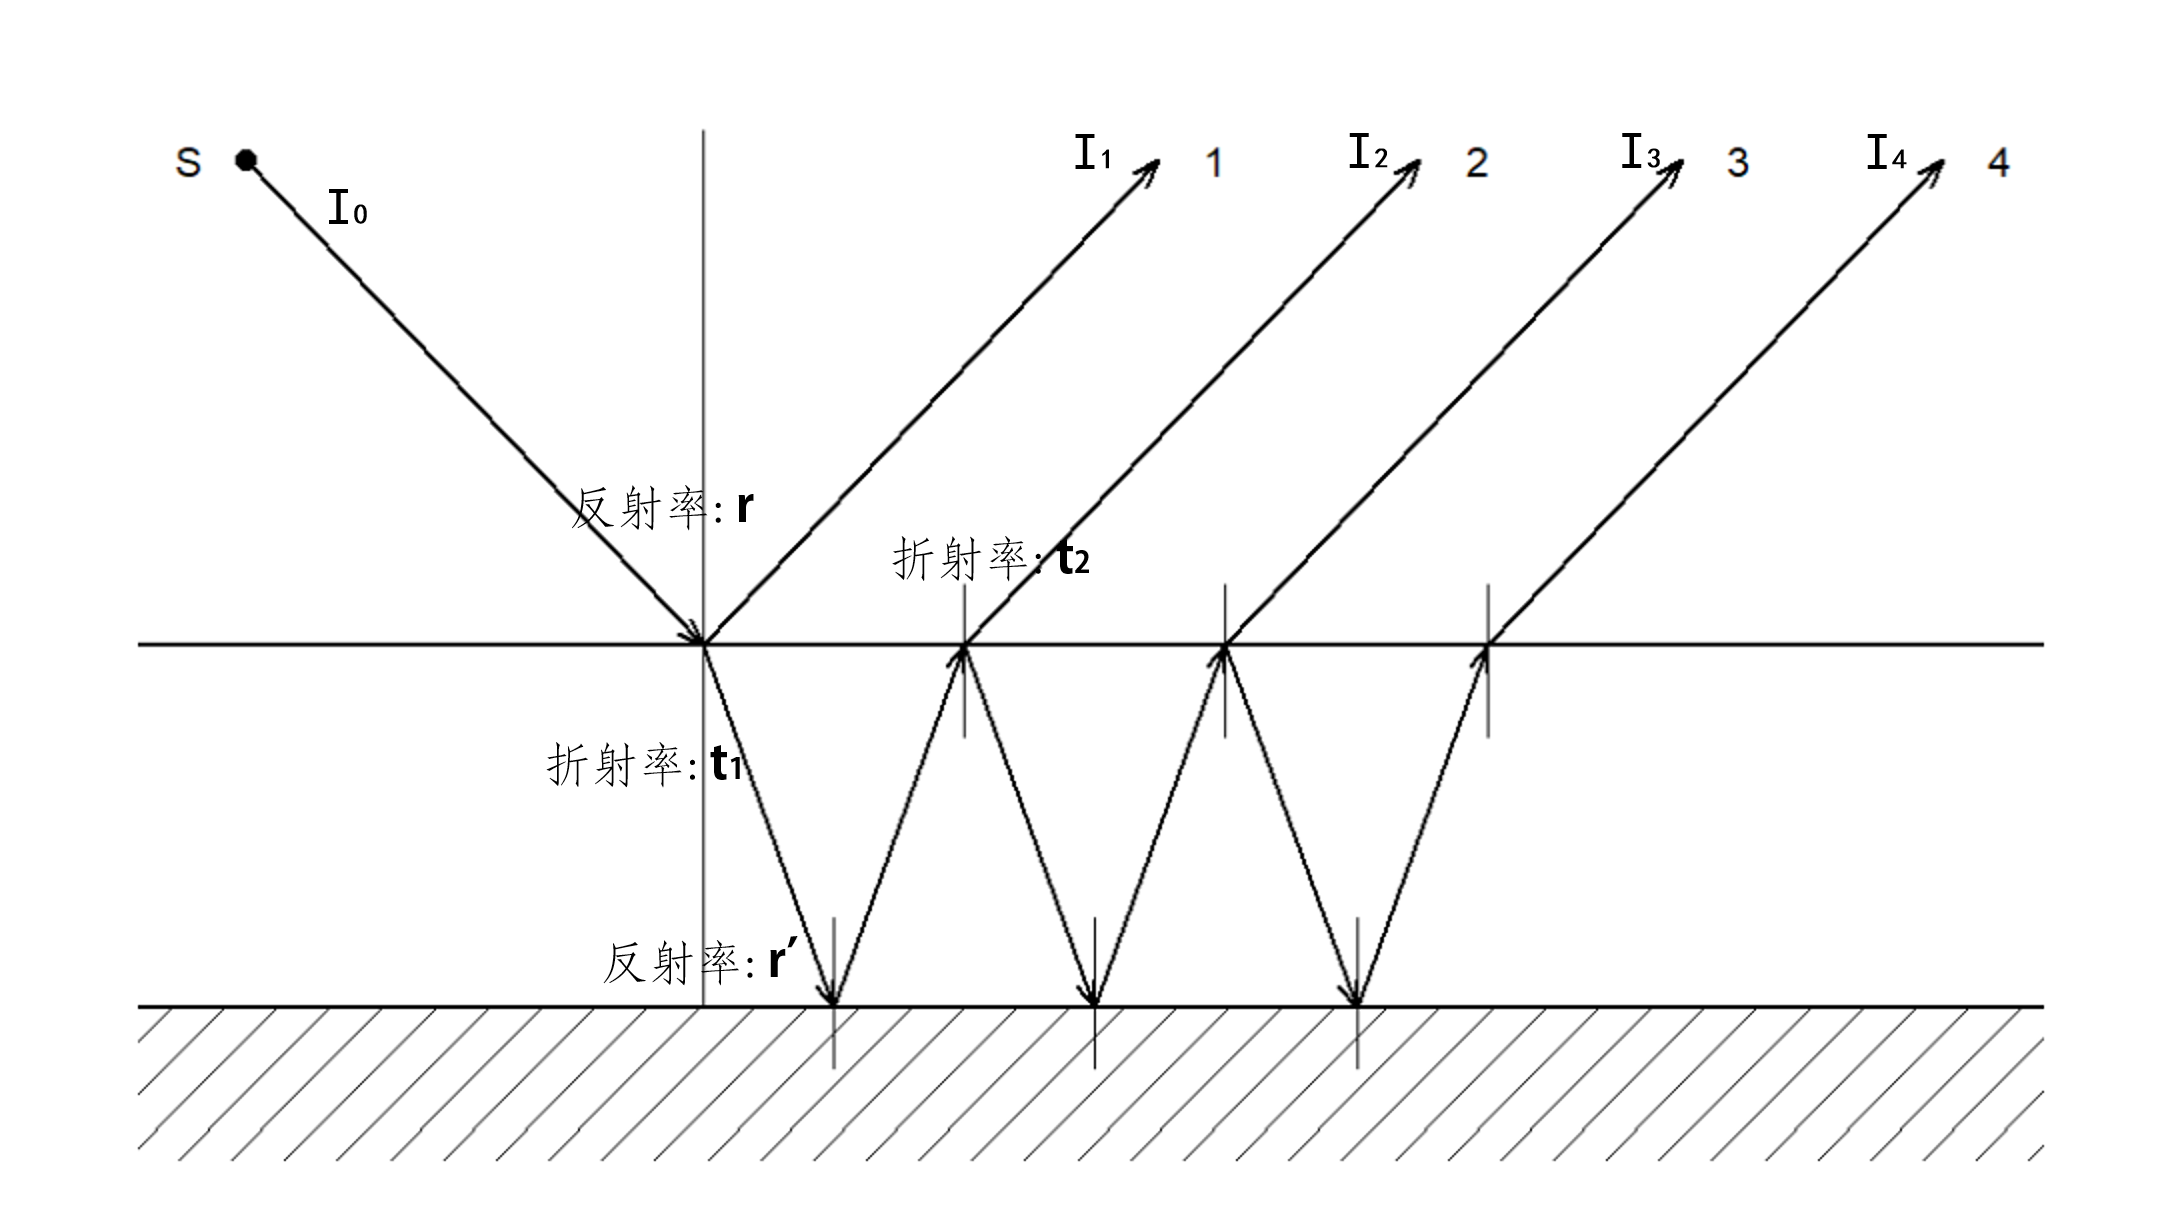
\includegraphics[width=1\linewidth]{4958a326605ed5ca76f5fb559fbfb7c7.png}
		\caption{}
	\end{figure}
\textbf{第1次反射光}(直接反射)光线直接从上层介质反射,仅经历1次反射:
		\[ I_1 = I_0 \cdot r \]
		\textbf{第2次反射光}(经下层界面反射后透射回来)两次透射,一次反射: \\
	    总光强为:
	    \[ I_2 = I_0 \cdot t_1 \cdot R' \cdot t_2  \]
	    \textbf{第3次反射光}经过两次透射,三次反射\\
	    总光强为:
	    \[ I_3 = I_0 \cdot t_1 \cdot R'^{(3)} \cdot t_2  \]
	    \textbf{第n次反射光}经过两次透射,(2n-3)次反射\\
	    总光强为:
	    \[ I_n = I_0 \cdot t_1 \cdot R'^{(2n-3)} \cdot t_2  \]
	    
	    多光干涉需保证后续反射光对干涉条纹有显著贡献,定义强度比阈值为 \( 0.1 \)(即后续光强不低于第1次反射光强的10\%)。
	    
	    第2次与第1次反射光强比
	    \[
	    \frac{I_2}{I_1} = \frac{I_0 \cdot t_1 \cdot r' \cdot t_2}{I_0 \cdot r} = \frac{t_1t_2 \cdot r'}{r} \geq 0.1
	    \]
	    代入能量守恒关系 \( t_1t_2 = 1 - r \):
	    \[
	    \frac{(1 - r) \cdot r'}{r} \geq 0.1 \tag{5}
	    \]
	    
	    第3次与第1次反射光强比
	    \[
	    \frac{I_3}{I_1} = \frac{I_0 \cdot t_1 \cdot r'^3 \cdot t_2}{I_0 \cdot r} = \frac{t_1t_2 \cdot r'^3}{r} \geq 0.1
	    \]
	    同理代入 \( t_1t_2 = 1 - r \):
	    \[
	    \frac{(1 - r) \cdot r'^3}{r} \geq 0.1 \tag{6}
	    \]
	    通过查表,硅晶圆片的折射率稳定为$3.42 \pm 0.03$,得到反射率$0.3  \pm 0.002$。
	    计算得出第3次反射光强仍然可以有不小的影响,无法忽略。
	\item \textbf{相位差稳定:}  
	  
	多束反射光的相位差需要保持固定值,才能形成稳定的干涉条纹。相位差由两部分组成:\\
	 光程差造成的相位差:
	 光程差导致的相位差公式为:
	 \[
	 \delta = \frac{2\pi}{\lambda} \cdot 2nd \cos(\theta) = \frac{4\pi nd \cos(\theta)}{\lambda}
	 \]
	 
	 其中:
	 - \(n\) 是介质的折射率,
	 - \(d\) 是光程差对应的路径长度,
	 - \(\theta\) 是入射角。
	 
	 反射相位差
	 
	 当光波从空气传播到外延层介质时,反射光会有相位差,这个相位差与光波的入射角、外延层的折射率 \(n_1\) 和衬底的折射率 \(n_2\) 相关。反射光的相位差受入射角的影响,不同的入射角产生不同的相位差。
	 
	 对于空气-外延层的界面,假设光波由介质1(空气,折射率为 \(n_1 = 1\))传播到介质2(外延层,折射率为 \(n_2\))时,反射的相位差 \(\Delta \Phi\) 可以通过以下公式计算:
	 
	 \begin{equation}
	 \Delta \Phi = \frac{4\pi n_2 d \cos(\theta)}{\lambda}\tag{16}
	 \end{equation}
	 
	 
	 
	
	    
\end{enumerate}
\subsection{模型建立}
\subsubsection{厚度计算 算法}
为定量对空气-外延层-衬底三层结构在多光谱光线照射下的干涉行为进行建模,我们首先将系统抽象为折射率分别为 \(n_0=1\)、\(n\)、\(n_\mathrm{c}\) 的三均匀平行平面,其中外延层厚度 \(d\) 为待测几何参数。设单色平面波以入射角 \(\theta_0\) 自空气入射,在外延层内折射角为 \(\theta\),满足斯涅尔定律 \(n_0\sin\theta_0=n\sin\theta\);衬底内折射角为 \(\theta_\mathrm{c}\),同理有 \(n\sin\theta=n_\mathrm{c}\sin\theta_\mathrm{c}\)。查询资料显示\upcite{franta2017temperature},单晶硅在$400\sim4000\ \mathrm{cm}^{-1}$处的折射率为$3.42\pm0.03$,可以认为其折射率不随波数变化。

根据菲涅尔公式,非偏振光在空气-外延层界面的振幅反射系数为
\begin{equation}
	\begin{split}
	R = \frac{K}{K + 1} = &\frac{1}{2}\bigg[ \left( \frac{n_1 \cos\theta_i - \sqrt{n_2^2 - n_1^2 \sin^2\theta_i}}{n_1 \cos\theta_i + \sqrt{n_2^2 - n_1^2 \sin^2\theta_i}} \right)^2 + \\
	&\left( \frac{n_2^2 \cos\theta_i - n_1 \sqrt{n_2^2 - n_1^2 \sin^2\theta_i}}{n_2^2 \cos\theta_i + n_1 \sqrt{n_2^2 - n_1^2 \sin^2\theta_i}} \right)^2 \bigg]
	\end{split}\tag{14}
	\end{equation}
外延层-衬底界面相应系数记为 \(r_{2s}\)、\(r_{2p}\),透射系数 \(t\)、\(t'\)、\(t_2\) 由能量守恒 \(t t'=1-r^2\) 及 Stokes 关系给出。考虑外延层内往返一次引入的光程差 \(\Delta L=2 n d \cos\theta\),对应相位差
\begin{equation}
\phi=\frac{2\pi}{\lambda}\Delta L=\frac{4\pi n d \cos\theta}{\lambda}.
\end{equation}
将空气-外延层界面的首次反射与外延层-衬底界面的多次反射相干叠加,得到复振幅级数
\begin{equation}
\mathcal{R}=r + t t' r_2 \mathrm{e}^{\mathrm{i}\phi} + t t' r_2^2 r \mathrm{e}^{2\mathrm{i}\phi} +\dotsb
\end{equation}
利用几何级数求和并代入能量守恒关系,化简得总反射率
\begin{equation}
R=|\mathcal{R}|^2=\frac{r^2+r_2^2+2 r r_2\cos\phi}{1+r^2 r_2^2+2 r r_2\cos\phi},
\end{equation}
同理总透射率
\begin{equation}
T=\frac{(1-r^2)(1-r_2^2)}{1+r^2 r_2^2+2 r r_2\cos\phi}.
\end{equation}
观察式(19)可得,多光束干涉的图象周期与$cos\phi$的周期相同,即多波束干涉的周期同样符合双波束干涉中的周期。因此,我们可以采用与第二问相似的算法计算外延层的厚度。
\subsubsection{多波束干涉的判定即性质利用}
多波束干涉的反射率函数形式如式(18)所示,因此函数图象的波动与双波束干涉图象不同:双波束干涉图象的波动上下对称,多波束干涉通常会出现上下波动不对称的情况,呈现出尖锐的波峰和相对平坦的波谷(或反之),如图所示
\begin{figure}[H]
		\centering
		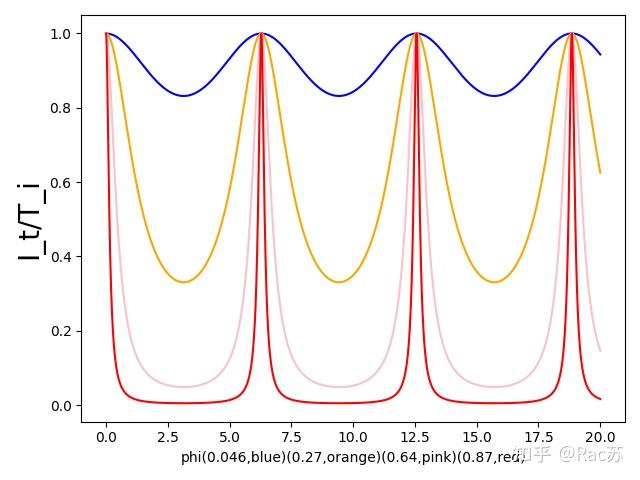
\includegraphics[width=.6\linewidth]{v2-c8a16483c780535fc84db696d14b227e_1440w.jpg}
		\caption{典型多波束干涉图象,图源网络\upcite{zhi2021juejin}}

	\end{figure}
为定量区分双光束与多光束干涉,本文将反射率–波数曲线视为一维信号,构造其
二阶导数 $R''(\tilde{\nu})$ 作为判据。
若曲线呈上下对称的类正弦振荡,则 $R''(\tilde{\nu})$ 的分布呈关于$0$轴对称;
若出现尖锐峰–平缓谷(或相反)的不对称特征,则 $R''(\tilde{\nu})$ 的分布呈关于$0$不对称。

在多波束薄膜干涉中,尖锐的波峰对应相长干涉条件精确满足的位置,此时多次反射光因相位一致而相干叠加,后继反射光与前导反射光同相增强,形成极高强度的干涉极大值。设薄膜折射率为 $n$,厚度为 $d$,入射角为 $\theta$,则相邻光束相位差为 $\delta = \frac{4\pi n d \cos\theta}{\lambda}$;当 $\delta = 2\pi m$($m \in \mathbb{Z}$)时发生相长干涉,反射光振幅叠加满足 $E_{\text{总}} = E_0 \sum_{k=0}^{\infty} r^k e^{i k \delta}$,强度为 $I \propto \left| \frac{1}{1 - r e^{i\delta}} \right|^2$,在 $\delta = 2\pi m$ 处分母最小,故 $I$ 出现尖锐极大值。

由于这个性质,我们能够更加精确地找到多波束干涉图象中的波峰位置,从而精确地确定多波束干涉的周期。

\subsection{模型求解}
\subsubsection{数据处理}
通过与第二问类似的算法,我们将反射率–波数曲线分解为趋势部分和波动部分。由于波动的不均匀性,我们换用STL分解方法对波动部分进行处理,结果如图。
\begin{figure}[H]
  \centering
  \begin{subfigure}[b]{0.49\linewidth}
    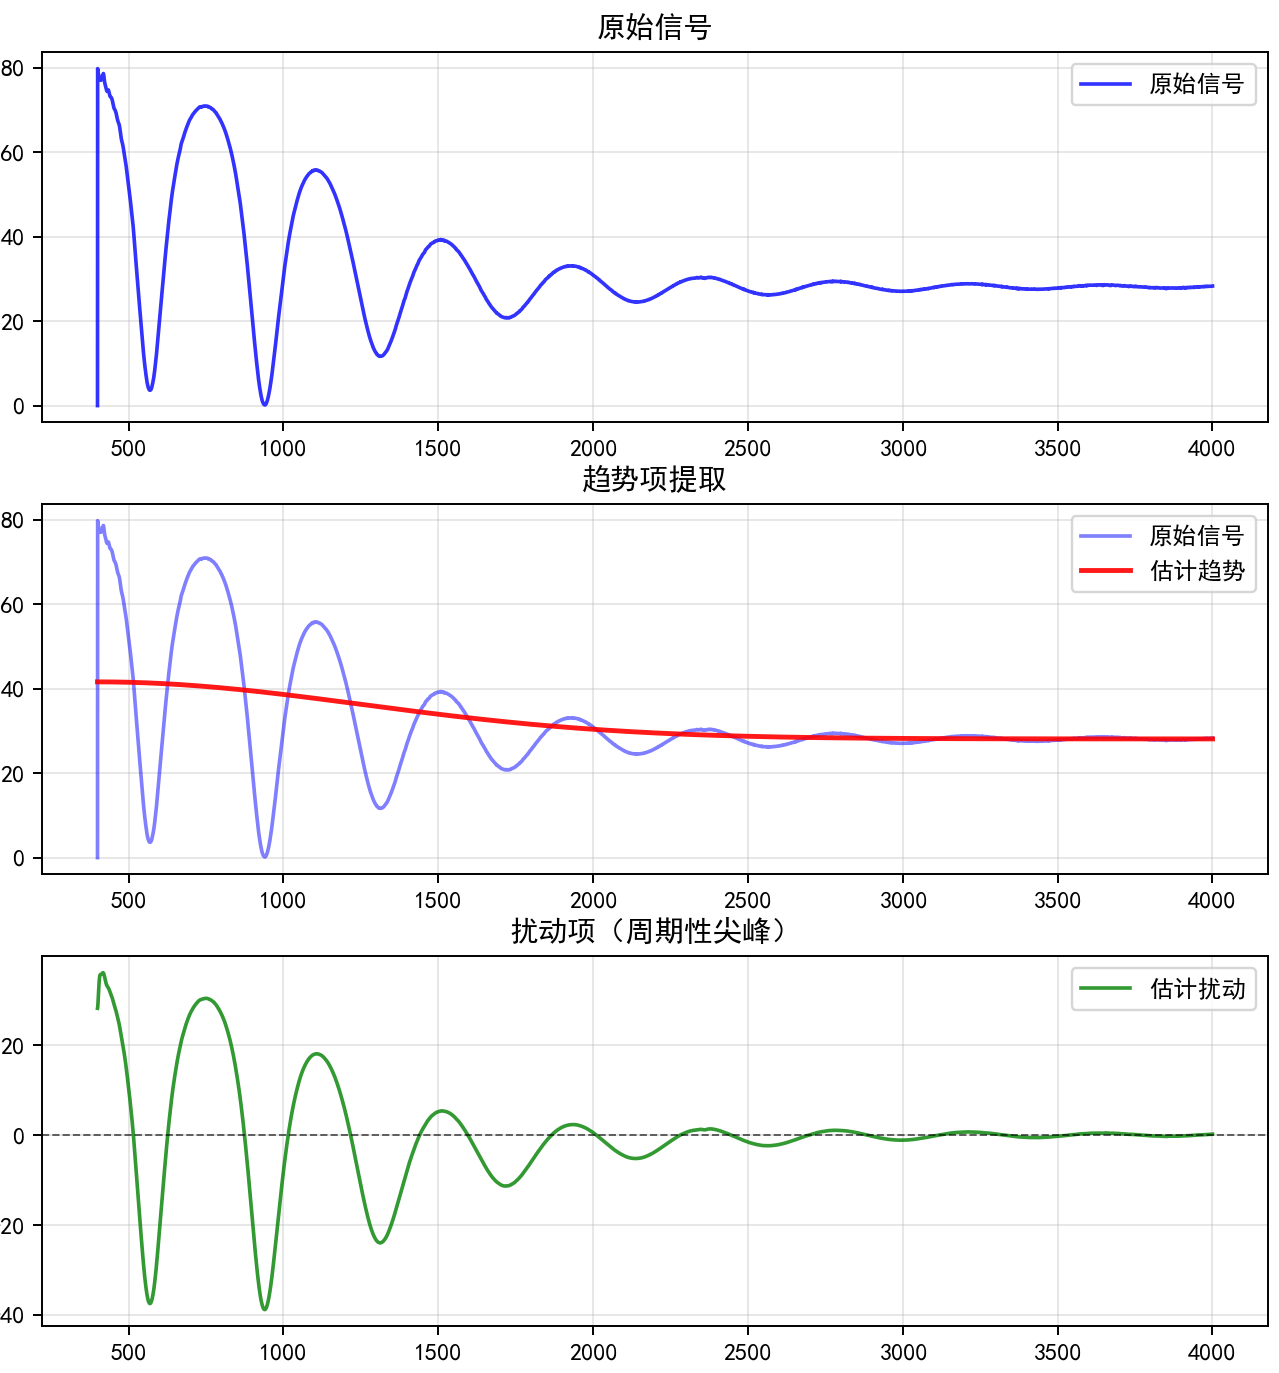
\includegraphics[width=\linewidth]{屏幕截图 2025-09-07 173211.png}

    \caption{附件3 反射率数据处理}
    \label{fig:附件3 反射率数据}
  \end{subfigure}
  \hfill
  \begin{subfigure}[b]{0.49\linewidth}
    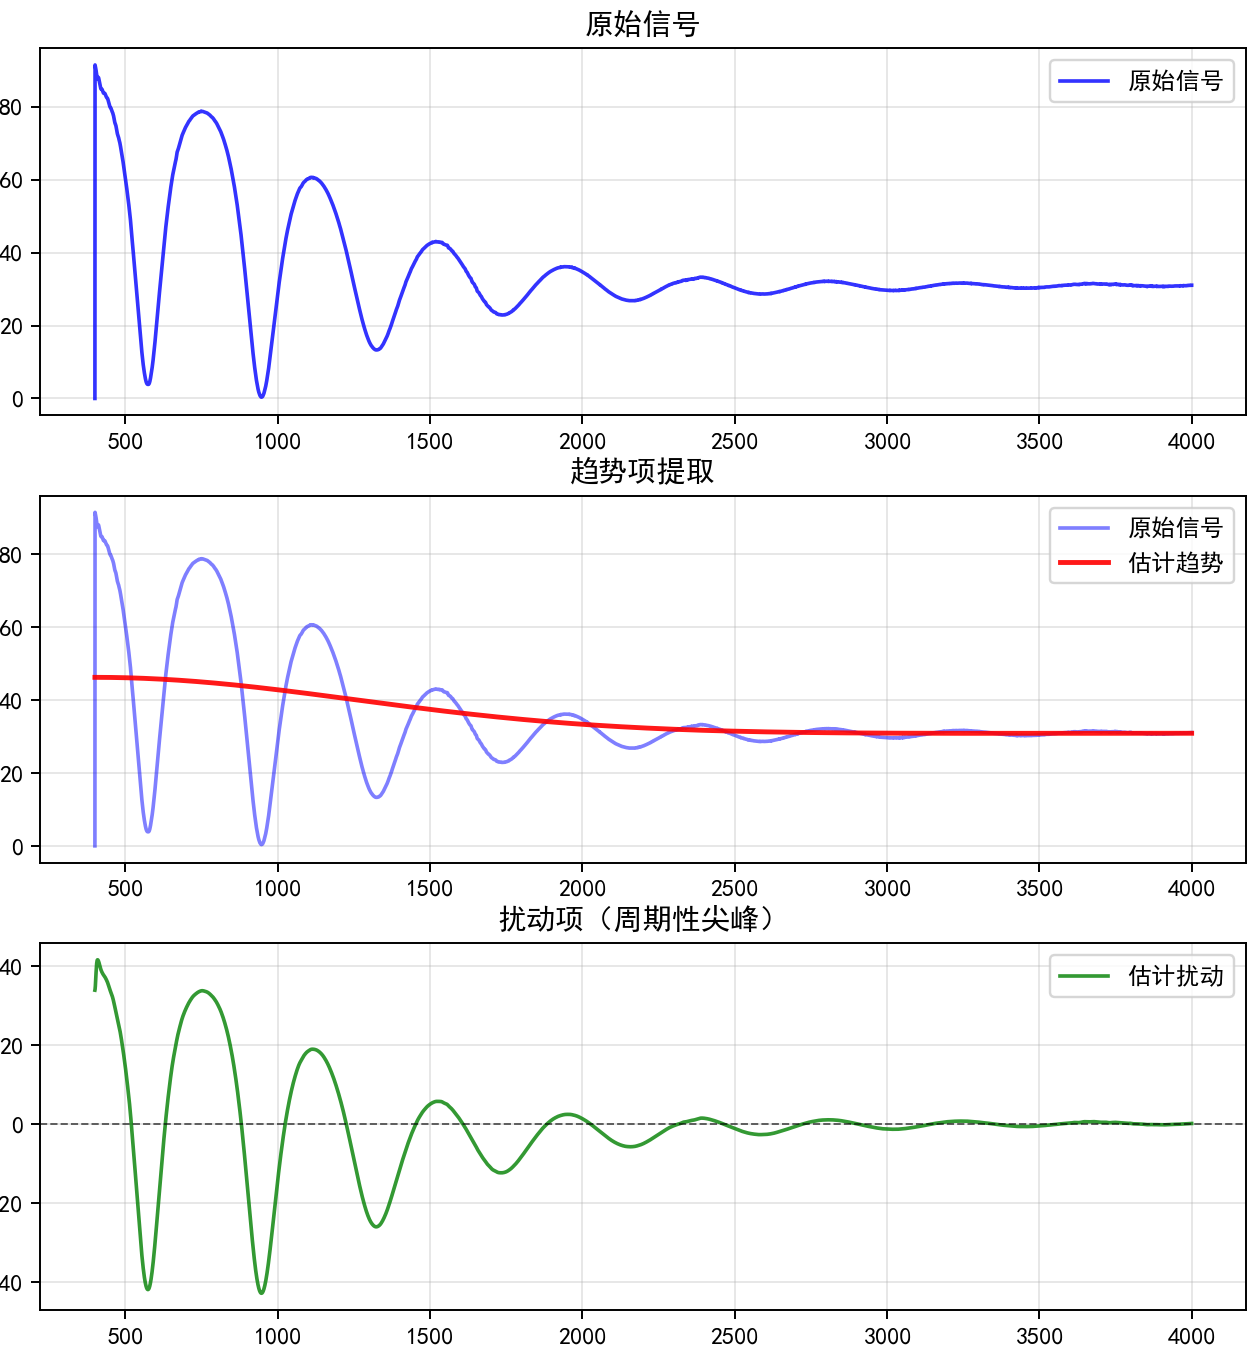
\includegraphics[width=\linewidth]{屏幕截图 2025-09-07 173239.png}
    \caption{附件4 反射率数据处理}
    \label{fig:maosniow}
  \end{subfigure}
  \caption{反射率数据处理}
  \label{fig:double4}
\end{figure}
然后,我们对分离出来的波动数据进行求导,得到波动的二阶导数。
\begin{figure}[H]
  \centering
  \begin{subfigure}[b]{0.8\linewidth}
    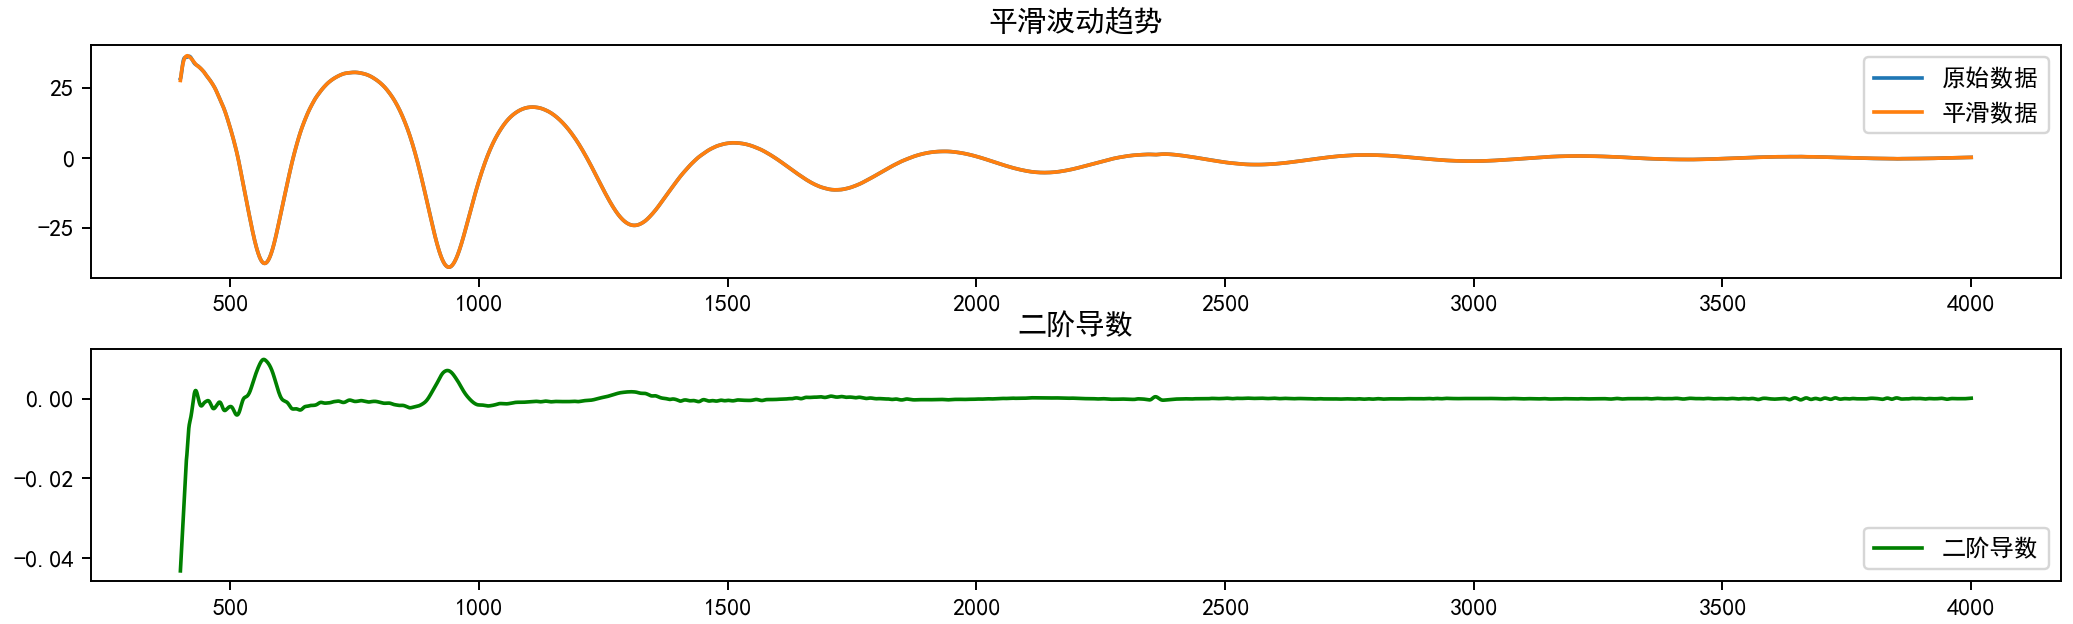
\includegraphics[width=\linewidth]{屏幕截图 2025-09-07 180041.png}
    \caption{附件3 求导结果}
    \label{fig:附件3 求导结果}
  \end{subfigure}
  \hfill
  \begin{subfigure}[b]{0.8\linewidth}
    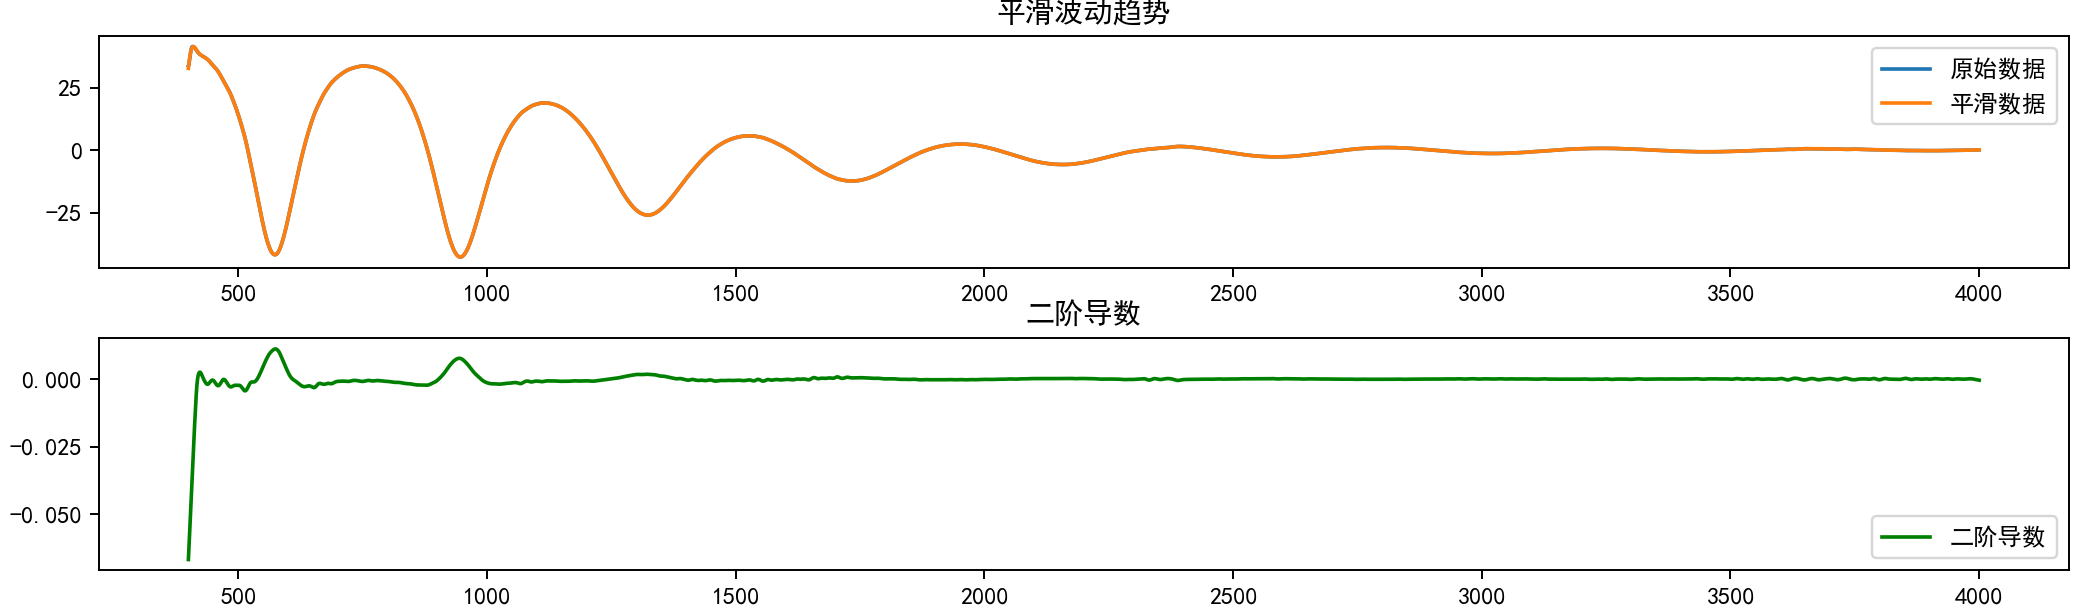
\includegraphics[width=\linewidth]{屏幕截图 2025-09-07 180102.png}
    \caption{附件4 求导结果}

    \label{fig:maosgniow}
  \end{subfigure}
  \caption{}
  \label{fig:double5}
\end{figure}

观察导数图象可得,在图象前两个波出现了较为明显的多波束干涉现象。由于发生多波束干涉将提高周期识别的准确性,因此我们使用两附件中前两个周期的数据求解。
\subsection{求解结果}
四个独立计算结果依次为
\[
d_1 = 3.9561\ \mu\text{m},\quad
d_2 = 3.9345\ \mu\text{m},\quad
d_3 = 3.9294\ \mu\text{m},\quad
d_4 = 3.8880\ \mu\text{m}.
\]
取平均值 $\bar{d}=3.9270\ \mu\text{m}$ 作为最终厚度估计。
以 $\bar{d}$ 为基准计算决定系数
\[
R^2 = 1-\frac{\sum_{i=1}^{4}(d_i-\bar{d})^2}
               {\sum_{i=1}^{4}(d_i-\bar{d})^2 + 4(\bar{d}-\bar{d})^2}
        = 0.9968,
\]
$R^2\approx0.997$ 表明模型拟合优度极高,数据波动仅由微小测量噪声引起,验证了算法的可靠性。
\subsection{附件1、2的多波束分析}
将附件1、2的数据通过求导处理\upcite{qwenmaxpreview2025},如图所示。

\begin{figure}[H]
  \centering
  \begin{subfigure}[b]{0.8\linewidth}
    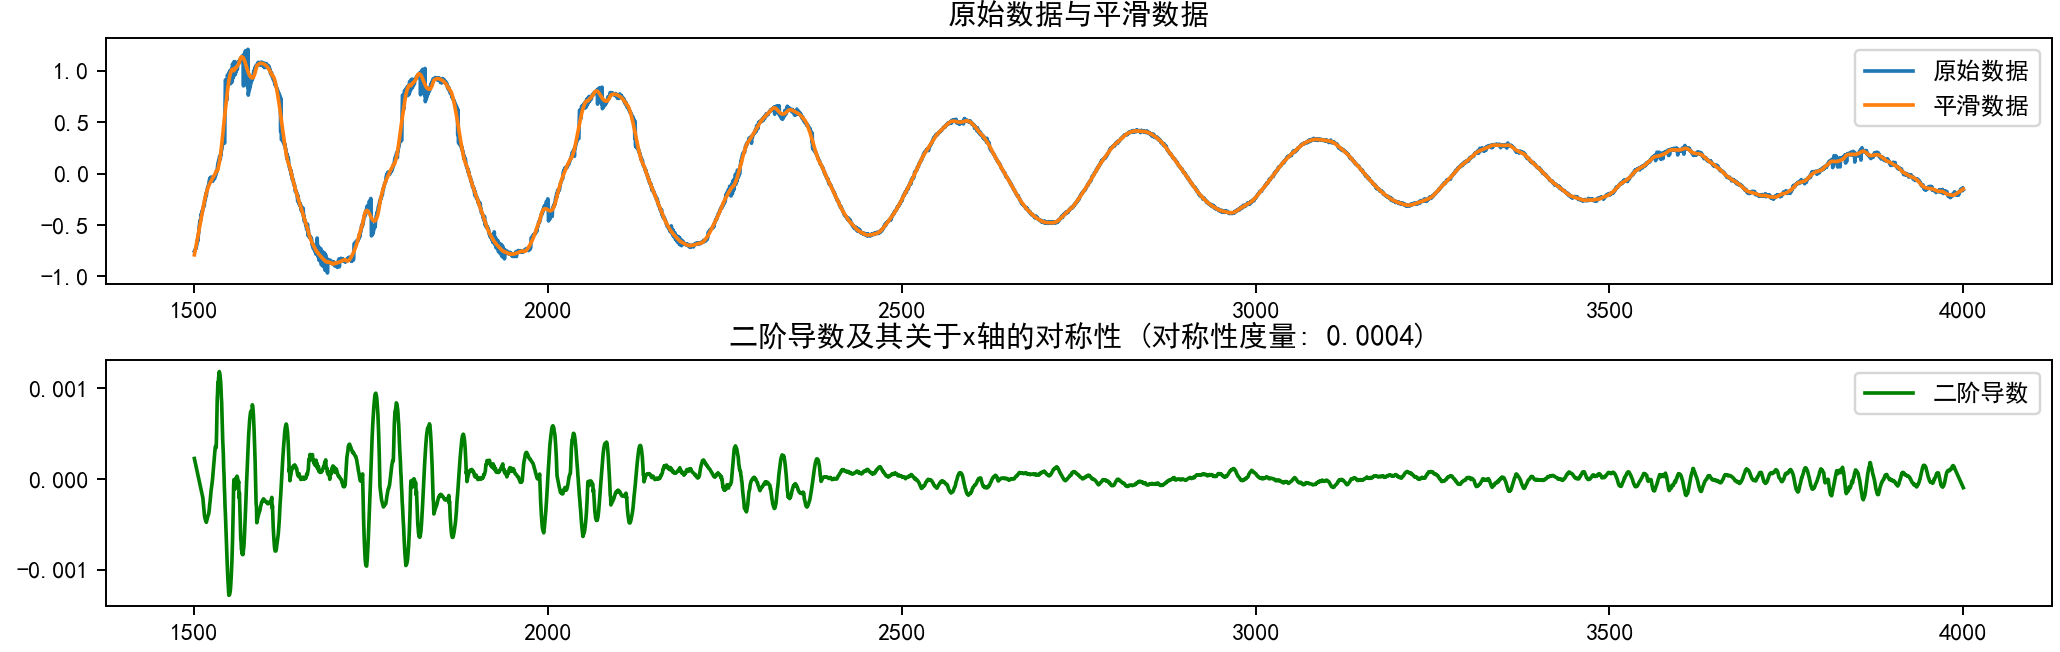
\includegraphics[width=\linewidth]{屏幕截图 2025-09-07 181935.png}
    \caption{附件1 求导结果}
    \label{fig:附件53 求导结果}
  \end{subfigure}
  \hfill
  \begin{subfigure}[b]{0.8\linewidth}
    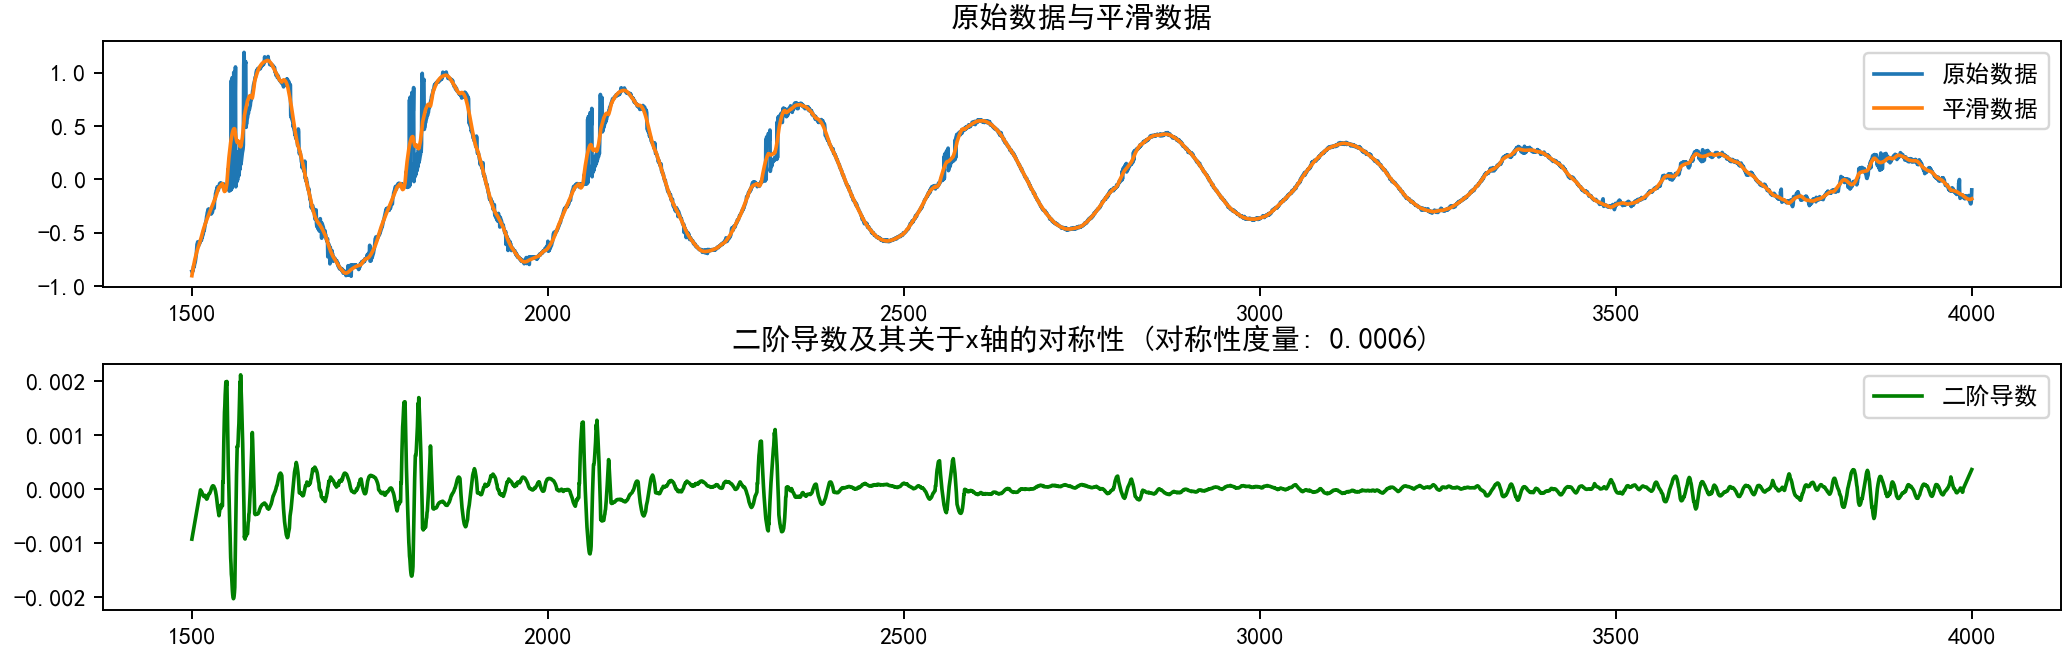
\includegraphics[width=\linewidth]{屏幕截图 2025-09-07 181955.png}
    \caption{附件2 求导结果}

    \label{fig:mao5sgniow}
  \end{subfigure}
  \caption{}
  \label{fig:double55}
\end{figure}
对以上的二阶导图象采用对称翻转后与原曲线进行均方根误差比较,发现二者的差异度均在$10**-3$一下,说明他们的曲线对称性良好。因此,我们认为SiC的外延层发生多波束干涉对于干涉曲线的影响可以忽略不计。

%%%%%%%%%%%%%%%%%%%%%%%%%%%%%%%%%%%%%%%%%%%%%%%%%%%%%%%%%%%%%

\bibliographystyle{gbt7714-numerical}  % 引用格式
\bibliography{ref}  % 引用 ref.bib 文件,无需写 .bib 后缀


\newpage
%%%%%%%%%%%%%%%%%%%%%%%%%%%%%%%%%%%%%%%%%%%%%%%%%%%%%%%%%%%%%
%% 附录
\begin{appendices}
\section{文件列表}
\begin{table}[H]
\centering
\begin{tabularx}{\textwidth}{LL}
\toprule
文件名  & 代码功能 \\

\midrule
傅里叶变换.py & 特征提取及高斯滤波 \\
最终boss.py & 厚度计算\\
boss二阶段.py & 厚度计算\\
菲涅尔定律计算折射率.py & 菲涅尔公式处理折射率文件\\
多波束数据处理 copy.py & 多波束数据处理\\
求导图象.py & 求导处理\\

\bottomrule
\end{tabularx}
\label{tab:文件列表}
\end{table}
\section{代码}

% -----------------  1  -----------------
\noindent\textbf{傅里叶变换.py}
\lstinputlisting[language=python]{code/傅里叶变换.py}

% -----------------  2  -----------------
\noindent\textbf{最终boss.py}
\lstinputlisting[language=python]{code/最终大boss.py}

% -----------------  3  -----------------
\noindent\textbf{boss二阶段.py}
\lstinputlisting[language=python]{code/boss二阶段.py}

% -----------------  4  -----------------
\noindent\textbf{菲涅尔定律计算折射率.py}
\lstinputlisting[language=python]{code/菲涅尔定律计算折射率喵.py}

% -----------------  5  -----------------
\noindent\textbf{多波束数据处理 copy.py}
\lstinputlisting[language=python]{code/多波束数据处理 copy.py}

% -----------------  6  -----------------
\noindent\textbf{求导图象.py}
\lstinputlisting[language=python]{code/求导图象.py}

\end{appendices}
\end{document}